\documentclass[12pt,a4paper]{article}
\addtolength{\textwidth}{1.5cm} 
\addtolength{\textheight}{1cm} 
\usepackage[T1,plmath]{english}
\usepackage{palatino}				% czcionka palatino
\usepackage[utf8]{inputenc}
\usepackage[pdftex]{graphicx}
\usepackage{amsmath}					% matematyka
\usepackage{url}
\usepackage[toc,page]{appendix}
\usepackage{slashbox}				% do podzielonej na pol komorki w~tabeli
\usepackage{fancyhdr}				% do nagłówkow, linia w~nagłówku
\usepackage{longtable}				% duze tabele > 1 strona
\usepackage[splitrule]{footmisc}	% ustawienia stopki
\usepackage{rotating}				% do obracania obiektów
\usepackage{indentfirst}	% na nazwie sekcji pierwszy akapit ze wcieciem
%\usepackage{polski}
\usepackage[T1]{fontenc} %dziwna szerokosc czcionki
% \usepackage{a4wide} % marginesy mniejsze
\usepackage[english]{babel}
\usepackage[polish]{babel}

\usepackage[
breaklinks=true,
colorlinks=true,
citecolor=black,
linkcolor=black,
anchorcolor=black,
urlcolor=black
]{hyperref}						% linki w~spisie tresci, rysukacj etc.
\usepackage[all]{hypcap}	% czasami hyperref Ÿle podaje \ref

\usepackage{textcomp} %wymagane przez listings - upquote=true

\usepackage{listings}
\lstset{
    language=Java,
    basicstyle=\scriptsize,
    aboveskip={1.5\baselineskip},
    columns=fixed,
    showstringspaces=false,
    extendedchars=true,
    breaklines=true,
    tabsize=4,
    prebreak = \raisebox{0ex}[0ex][0ex]{\ensuremath{\hookleftarrow}},
    showtabs=false,
    showspaces=false,
    showstringspaces=false,
    identifierstyle=\ttfamily,
    keywordstyle=\color[rgb]{0,0,0},
    commentstyle=\color[rgb]{0,0,0},
    stringstyle=\color[rgb]{0,0,0},
    numbers=left,
    numberstyle=\tiny,
    stepnumber=1,
    numbersep=5pt,
    captionpos=b,
}

\renewcommand*\thelstnumber{\the\value{lstnumber}:} % dwukropek po numerze linii

%\usepackage[small,bf]{caption} % mniejsza czcionka dla podpisów

\sloppy		% mniej staranne łamanie wierszy, zapobiega wystawaniu wyrazom po za 
% szaltę dokumentu

\headheight=15pt
\pagestyle{fancy}
\fancyhead[R]{\small \thepage}
\fancyhead[C]{\small \leftmark}
\fancyhead[L]{}
\fancyfoot{}
\renewcommand{\sectionmark}[1]{%
\markboth{\thesection.\ #1}{}}
\renewcommand{\headrulewidth}{0.4pt}
\renewcommand{\footrulewidth}{0.4pt}


\renewcommand{\textfraction}{0.05}
\renewcommand{\baselinestretch}{1.05}

\newcommand{\ninter}{\renewcommand{\baselinestretch}{1.5}}
\newcommand{\sinter}{\renewcommand{\baselinestretch}{1.0}}
\newcommand{\eng}[1]{(ang.\ \emph{#1})}
\renewcommand\labelitemi{\textbullet}
\renewcommand\labelitemii{$\circ$}  
\renewcommand\labelitemiii{---} %{\textasteriskcentered}
\renewcommand\labelitemiv{---}  %{\textperiodcentered} 

\renewcommand\figurename{Fig.}
\renewcommand\tablename{Table}
\renewcommand\lstlistingname{Listing}
\renewcommand\lstlistlistingname{Code listing}

\makeatletter
\renewcommand{\fnum@table}{\textbf{\tablename~\thetable}}
\makeatother

% numerowaie obrazkow 1.1 1.2 1.3... 2.1 2.2 2.3
\renewcommand{\thefigure}{\arabic{section}.\arabic{figure}}
\renewcommand{\theequation}{\arabic{section}.\arabic{equation}}
\let\stdsection\section
\renewcommand\section{\setcounter{figure}{0}\setcounter{equation}{0}\setcounter{table}{0}\setcounter{lstlisting}{0}\stdsection}

%numerowanie tabel
\renewcommand{\thetable}{\arabic{section}.\arabic{table}}


%%%%%%%COUNTER DO TABEL%%%%%%%%%
%\newcounter{tableindex}
%\newcommand{\tindex} { \thetableindex \stepcounter{tableindex} }
%DOCUMENT%%%%%%%%%%%%%%%%%%%%%%%%%%%%%%%%%%%%%%%%%%%%%%%%%%%%%%%%%% 

%%%%%%%%TO~NALEZY UZUPELNIC%%%%%%%%%%%%%%%%
\def\temat{Efficiency evaluation of parallel genetic algorithms and
evolutionary programs}
\def\tematen{Badanie efektywności równoległej realizacji algorytmów genetycznych
i programów ewolucyjnych}
\def\autor{Marcin Majak}
\def\prowadzacy{Leszek Koszałka, PhD, W4/K2}
\def\opiekun{dr inż. Leszek Koszałka, W4/K2}
\def\rok{2010}

\newcommand{\mojaSugestia}[1]{\textcolor{blue}{#1}}
\newcommand{\mojaZmiana}[1]{\textcolor{green}{#1}}
\newcommand{\kodWTexcie}[1]{\texttt{#1}}

\usepackage{placeins}  % to many unprocessed floats - problem z numerowaniem wiecej niz 20 obrazkow

\begin{document}

%numerowanie listingów
\renewcommand{\thelstlisting}{\arabic{section}.\arabic{lstlisting}}

%po wpisaniu makr przed \begin{document} strona
%tytulowa uzupelni sie automatycznie

%Mon Dec 18 16:18:58 CET 2006
%autor: Krystian Piećko
\titlepage
%\addtolength{\hoffset}{-1cm}
\addtolength{\textheight}{1.8cm}
%\addtolength{\footskip}{-2cm}
\addtolength{\textwidth}{0.2cm}
%\addtolength{\oddsidemargin}{-1.2cm}
\addtolength{\topmargin}{-2.2cm}
\enlargethispage{3cm}
\begin{center}
	\begin{Huge}
		\textsc{Politechnika Wrocławska}
	\end{Huge}

	\begin{huge}
		\vspace{1ex}
		\textsc{Wydział Elektroniki}
	\end{huge}
	\rule[-0.3ex]{\textwidth}{1pt}
	
	\begin{flushleft}
		\begin{large}
			\vspace{0.4cm}
			\textsc{Kierunek: Informatyka (ang.)} \newline
		\end{large}
	\end{flushleft}

	\begin{center}
		\begin{Huge}
			\vspace{1.7ex}
			\textsc{\textbf{Praca magisterska}} 

		\end{Huge}
	\end{center}
	\vspace{1cm}
		
	%\vspace{1.5cm}
	\begin{flushright}
		\begin{minipage}[t][4cm][t]{11cm}
			\begin{center}
				\begin{large}
					\tematen
				\end{large}
			\end{center}
			%\newline
			\vspace{0.3cm}
			\begin{center}
				\begin{large}
					\temat
				\end{large}
			\end{center}
		\end{minipage}
	\end{flushright}
				
	\begin{flushright}
		\begin{minipage}[t]{10cm}
			\begin{flushleft}
				\begin{large}
					%\vspace{2ex}
					\vspace{0.3cm}
					\begin{large}
						\textsc{Autor:}\newline
						\autor\newline
					\end{large}
					
					\vspace{1.5cm}
					\textsc{Opiekun:}\newline
					\opiekun\newline
					
					\vspace{0.5cm}
					\textsc{Ocena pracy:}\newline
				\end{large}
			\end{flushleft}
		\end{minipage}
	\end{flushright}
	\vfill
	\rule[-0.3ex]{\textwidth}{1pt}
	WROCŁAW \rok
\end{center}
\newpage
\clearpage
\enlargethispage{-3cm}
\addtolength{\textheight}{-1.8cm}
\addtolength{\textwidth}{-0.2cm}
\addtolength{\topmargin}{2.2cm}


\newpage
\selectlanguage{polish}
\begin{center}
	Streszczenie
\end{center}

Niniejsza praca porusza problem równoległej realizacji algorytmów genetycznych
i~procesów ewolucyjnych. W ostatnich czasach nastąpił znaczący rozwój komputerów
wieloprocesorowych, dzięki czemu pojawiła się możliwość prowadzenia obliczeń
rozproszonych; jako przykład można podać ``cloud computing'' czy też struktury
meshowe. Analizę równoległej realizacji algorytmów można przeprowadzić na dwóch
płaszczyznach: pierwsza to rozkład struktury algorytmu i wydzielenie części, które
mogą zostać zrealizowane równolegle, a także określenie opłacalności tego
zrównoleglenia; druga płaszczyzna to implementacja algorytmu i wybór
odpowiedniego środowiska do testowania. 

Przeprowadzone symulacje skupiają się na zbadaniu efektywności realizacji
równoległego algorytmu genetycznego w stosunku do wersji sekwencyjnej,
szczególnie pod kątem czasu trwania algorytmu, a także uzyskanej dokładności
rozwiązania. Algorytm genetyczny został wzięty do analizy ze względu na
swoją budowę i łatwość zrównoleglenia pewnych operacji, takich jak mutacja,
reprodukcja. Aby przeprowadzić wszystkie symulacje, został napisany program w
języku C++ symulujący prosty sekwencyjny algorytm genetyczny, a także jego
równoległy odpowiednikm, gdzie migracja odbywa się na dwa sposoby: w~pierwszym
przypadku tylko do jednego sąsiada danego procesu slave, natomiast w~drugim do
dwóch sąsiednich procesów slave jednocześnie. Do testowania zostały wykorzystane
dobrze znane w~literaturze przedmiotu funkcje testowe, m.in. funkcje De Jong'a,
ze wględu na swoją różnorodność, a~także występowanie kilku wartości lokalnego
minimum ale tylko jednego globalnego co znacznie utrudnia znalezienie właściwej
wartości przy małej różnorodności osobników. 
Zadaniem stworzonego algorytmu było znalezienie minimum danej funkcji w~określonym przedziale.
Z~racji tego, że znane było globalne minimum pojawiła się możliwość
jednoznacznej oceny wydajności algorytmów za pomocą zaproponowanych wskaźników
efektywności:
\begin{itemize}
	\item Błąd bezwzględny pomiędzy znalezionym rozwiązaniem, a wartością
		a-priori globalnego minimum. Wyróżniono trzy wskaźniki:
		\begin{itemize}
			\item Najmniejsza wartość błędu z~$n$ symulacji 
				\begin{equation}
					B=MIN\left | f^{*}(\underline{x})-f(\underline{x}) \right |
					\label{min1}
				\end{equation}
			\item Największa wartość błędu z~$n$ symulacji 
				\begin{equation}
					W=MAX\left | f^{*}(\underline{x})-f(\underline{x}) \right |
					\label{min3}
				\end{equation}
			\item Średnia wartość błędu z~$n$ symulacji
				\begin{equation}
					A=\frac{1}{n}\sum_{n=1}^n\left | f^{*}(\underline{x})-f(\underline{x}) \right |
					\label{min2}
				\end{equation}
		\end{itemize}
		gdzie $f^{*}(\underline{x})$ oznacza wartość funkcji wyznaczoną przez
		testowany algorytm, a~$f(\underline{x})$ to globalne minimum.
	\item Wariancja błędu z~$n$ symulacji 
		\begin{equation}
			\sigma^2=\frac{1}{n-1}\sum_{i=1}^n\left[A-B\right]^2
			\label{min4}
		\end{equation}
	\item Średni czas trwania algorytmu z~$n$ symulacji, gdzie $T_i$ to $i-ty$ 
		czas symulacji
		\begin{equation}
			T=\frac{1}{n}\sum_{i=1}^nT_i
			\label{min4}
		\end{equation}
\end{itemize}


Symulacje zostały przeprowadzone na platformie Linux z wykorzystaniem
oprogramowania pvm(Parallel Virtual Machine), które pozwala na wirtualizację
kilkunastu procesorów na jednej stacji roboczej pełniącej rolę mastera. W
przypadku algorytmów genetycznych bardzo ważną rolę odgrywają parametry
konfiguracyjne. Źle dobrane mogą wpłynąć znacznie na wydajność, szczególnie na
czas trwania algorytmu, a~także jakość znalezionego rowiązania. Często przed
przystąpieniem do symulacji parametry te ze względu na skomplikowane zależności
wybierane są losowo, jednak w tej pracy konfiguracja została ustalona na
podstawie literatury przedmiotu, analizując dostępne rozwiązania i rezultaty
zaprezentowanych aplikacji. Program stworzony na potrzeby tego projektu był
uruchamiany z wykorzystaniem lini komend, a~do kompilacji zdefiniowano reguły
w~pliku \tescsc{MAKEFILE}. Dokładniejszy opis programu i~wykorzystanych
bibliotek znajduje się w~dołączonym do pracy załączniku. 
Ze względu na stochastyczny charakter działania algorytmów genetycznych każda z
symulacji była powtórzona $200$~razy, a ostateczne wyniki uśredniono. 

Praca została podzielona na dwie części. Rozdziały 2~i~3 stanowią wprowadzenie
do tematyki równoległych algorytmów genetycznych; zostały tam opisane kryteria
podziału, a także sposoby równoległej realizacji wraz z matematycznym
uzasadnieniem opłacalności ich stosowania. Środowisko testowania, a~także
stworzony program zostały przedstawione w rozdziale~4, natomiast właściwe
wyniki badań wraz z komentarzem znajdują się w rozdziale~5. Zostały
wykorzystane tam dwa typy algorytmów genetycznych: pierwszy to prosty
sekwencyjny przypadek, natomiast drugi to implementacja realizująca równoległy
algorytm genetyczny z kilkoma subpopulacjami, określany w literaturze jako
``Gruboziarnisty równoległy algorytm genetyczny''. Symulacje miały na celu zbadanie
ogólnych zależności pomiędzy liczbą CPU, częstością migracji i~liczbą
osobników, a~także ich wpływ na efektywność algorytmu. Propozycje przyszłych
badań oraz ogólne podsumowanie pracy można znaleźć w rozdziałach 6~i~7.

Biorąc pod uwagę fakt, że projekt ten jest pierwszym w dziedzinie równoległej
realizacji algorytmów genetycznych, warto było na początku przeprowadzić
podstawowe badania które miały na celu nakreślić ogólny charakter algorytmów
równoległych w~stosunku do wersji sekwencyjnej, a~także wpływ parametrów
konfiguracyjnych. Przeprowadzone w tym projekcie badania symulacyjne skupiły się
głównie na trzech podstawowych ale bardzo ważnych aspektach realizacji algorytmów równoległych:
\begin{enumerate}
	\item Liczba CPU w stosunku do czasu trwania algorytmu, a~także jakości
		uzyskanego rozwiązania. W przypadku algorytmów genetycznych bardzo
		ważną rolę odgrywa narzut komunikacyjny, który w pewnym momecie może być
		nawet większy niż czas obliczenia funkcji przystosowania danego
		osobnika. 
	\item Częstość migracji- tutaj pojawia się pytanie jaka konfiguracja jest
		optymalna. Czy lepiej jest częściej dokonywać wymiany osobników aby ustrzec
		się przed zbyt szybką konwergencją, jednak z drugiej strony zbyt
		intensywna migracja zwiększa narzut komunikacyjny i~może prowadzić do
		zachwiania stabilności rozwiązania. 
	\item Liczba osobników biorących udział w procesie migracji- podobnie jak w
		poprzednim punkcie należy znaleźć balans pomiędzy narzutem
		komunikacyjnym, a~jakością otrzymanego rozwiązania i~czasem trwania
		algorytmu.
\end{enumerate}
Jak można zauważyć na podstawie powyższych punktów nawet podstawowe parametry
konfiguracyjne mają ogromny wpływ na wydajność algorytmu.

Przeprowadzone w tym projekcie badania potwierdziły, że aby zaimplementować wydajny równoległy
algorytm genetyczny parametry konfiguracyjne muszą być wybrane z dużą rozwagą.
Wiele rzeczy musi być wziętych pod uwagę, takich jak topologia, częstość
migracji czy też liczność populacji. Generalny wniosek płynący z przeprowadzonych 
eksperymentów to opłacalność stosowania $\mathcal{PGA}$, w stosunku do
$\mathcal{SGA}$, jednak należy tutaj podkreślić, że tylko w sytuacji dobrania
odpowiedniej konfiguracji wejściowej. W pracy zostały zaprezentowane przypadki,
w których nawet jeden niewłaściwie dobrany parametr negatywnie wpływał na
wydajność $\mathcal{PGA}$. Zbadany $\mathcal{CPGA}$ był w stanie znaleźć
generalnie o~wiele lepsze, w sensie
jakościowym, rozwiązania dla testowanych problemów optymalizacyjnych niż standardowy
$\mathcal{SGA}$. Prócz tego charakteryzował się ogólnie większą stabilnością, 
a~zatem i większą przewidywalnością i niezawodnością działania. Zjawisko to było
szczególnie widoczne w odniesieniu do problemów o względnie skomplikowanej naturze.

Podsumowując należy zaznaczyć, że niniejsza praca zrealizowała w całości
sformułowane cele, mianowicie: przedstawiona została jednolita systematyka występujących
w literaturze przedmiotu, współbieżnych implementacji $\mathcal{GA}$ wraz z
metodyką doboru konkretnego sposobu realizacji równoległej w zależności od
dostępnych zasobów. Opisana została teoretyczna analiza oczekiwanych ze zrównoleglenia
korzyści wraz z~matemtycznym uzasadnieniem oraz przeprowadzone zostały badania eksperymentalne
wybranej arbitralnie techniki realizacji równoległej, którą w tym przypadku
reprezentował algorytm $\mathcal{CPGA}.



\newpage

%Mon Dec 18 16:18:58 CET 2006
%autor: Krystian Piećko
\selectlanguage{english}
\titlepage
%\addtolength{\hoffset}{-1cm}
\addtolength{\textheight}{1.8cm}
%\addtolength{\footskip}{-2cm}
\addtolength{\textwidth}{0.2cm}
%\addtolength{\oddsidemargin}{-1.2cm}
\addtolength{\topmargin}{-2.2cm}
\enlargethispage{3cm}
\begin{center}
	\begin{Huge}
		\textsc{Wroclaw University of Technology}
	\end{Huge}

	\begin{huge}
		\vspace{1ex}
		\textsc{Faculty of Electronics}
	\end{huge}
	\rule[-0.3ex]{\textwidth}{1pt}
	
	\begin{flushleft}
		\begin{large}
			\vspace{0.4cm}
			\textsc{AREA: Teleinformatic(TIN)} \newline
		\end{large}
	\end{flushleft}

	\begin{center}
		\begin{Huge}
			\vspace{1.7ex}
			\textsc{\textbf{Engineering project}} 

		\end{Huge}
	\end{center}
	\vspace{1cm}
		
	%\vspace{1.5cm}
	\begin{flushright}
		\begin{minipage}[t][4cm][t]{11cm}
			\begin{center}
				\begin{large}
					\temat
				\end{large}
			\end{center}
			\vspace{0.3cm}
			\begin{center}
				\begin{large}
					\tematen
				\end{large}
			\end{center}
		\end{minipage}
	\end{flushright}
				
	\begin{flushright}
		\begin{minipage}[t]{10cm}
			\begin{flushleft}
				\begin{large}
					%\vspace{2ex}
					\vspace{0.3cm}
					\begin{large}
						\textsc{Author:}\newline
						\autor\newline
					\end{large}
					
					\vspace{1.5cm}
					\textsc{Supervisor:}\newline
					\prowadzacy\newline
					
					\vspace{0.5cm}
					\textsc{Grade:}\newline
				\end{large}
			\end{flushleft}
		\end{minipage}
	\end{flushright}
	\vfill
	\rule[-0.3ex]{\textwidth}{1pt}
	WROCŁAW \rok
\end{center}
\newpage
\clearpage
\enlargethispage{-3cm}
\addtolength{\textheight}{-1.8cm}
\addtolength{\textwidth}{-0.2cm}
\addtolength{\topmargin}{2.2cm}


\newpage
\thispagestyle{empty}
\begin{center}
	Abstract
\end{center}

This paper concerns the problem of parallel genetics
algorithms and evolutionary programs realization. In the last few decades multiprocessor
computers have spawned development of dispere computation processes, to name
only the few it is cloud computing or mesh grid computers. Design of parallel
algorithms can be carried out in two steps. The first is algorithm's structure
analysis and distinction of processes which can be realised in parallel, with
additional consideration of parallelisation profitability. The second step involves algorithm's
implementation and testing environment setup.

Simulations are focused on efficieny analysis between
parallel genetic algorithm and its sequential counterpart, especially in case
of algorithm's duration and solution accuracy. Genetic algorithm was used
because of its structure and its simplicity to realised some methods in parallel
such as: mutation, reproduction, etc. To manage all the simulations program was
written in C++ simulating sequential and parallel genetic algorithms. For
testing, well known in the literature test functions were used mainly De Jong's
functions and in order to fairly evaluate results efficiency indicators were
proposed in this paper. 

All test were performed on Linux platform with the help of pvm(Parallel Virtual
Machine) framework, which allows virtualization of few processors on one machine
called master. Taking into account the stochastic nature of genetic algorithm
each simulation was repeated $200$ times and the final results represent the
average value. 

This paper is divided into two parts. Sections 2~and~3 are the introduction into
parallel genetic algorithm subject matter. There are listed types of parallel algorithm
and method of parallelisation with mathematical justification. Testing
environment setup and program used in simulations are described in section~4,
while the results of experiments with comments are placed in section~5. 
There were used two types of algorithms: the first is simple sequential while 
the second is parallel genetic algorithm with few subpopulations. The main 
goal of simulations was to find the relationship between number of slave units, 
the interval of migration and number of individuals and their impact on algorithm
efficiency. Proposal of future work as the continuation of this topic and the
final summary can be found in sections 6~and~7.


\newpage
\tableofcontents
\newpage

%od tego miejsca mozna zaczac wpisywac tresc.
%polecam korzystac z~polecenia input i~kazdy rozdzial robic w~innym pliku
%tak jak jest wciagnieta titlepage

\newpage
\section{Introduction}
\subsection{Preface}
\label{cha:Goals}
With the improvement of computers we are able to tackle with high dimensional 
problems in many areas of human life. At first glance everything
looks so easy, but when we go deeper into a problem more and more problems 
become evident and unavoidable. For example, reconsider pattern recognition
tasks in which measured objects (patterns) coming from the environment can be 
described by many attributes. Some of them are very meaningful while others brings only noise 
and distortion. This is the role of the algorithm to pick valuable attributes,
but finding a minimal attribute reduct is $\mathcal{NP}$-hard problem. Another
obstacle is connected with overlaps in the attribute space. When attributes 
are easily separable even a simple classifier works perfectly, but for more 
tricky cases very sophisticated approaches have to be applied.

For the past years, many scientist in the world tried to invent new algorithms
to simplify and improve the accuracy of classification. There are many solutions, 
but ones of the most eminent in the literature are: neural networks, fuzzy logic or 
evolutionary algorithms such as genetic algorithm or tabu search. 
Because simple approaches failed in more complicated problem, scientists tried
to apply algorithms for dimensionality reduction and merge abilities of single
classifier into combined one. This improved the quality of classification 
significantly, but until now no one has managed to invent such a classifier 
that will never make no mistakes.

This thesis touches the broad topic of pattern recognition task which is 
very difficult and demanding problem in every aspect of science. Generally, 
pattern classification is about assigning label to an unknown object based 
on the available knowledge coming from training dataset or expert experience.
This process be compared to the capability of human brain which is able to put 
certain scenario into context and identify distinguishable object components. 
The whole process of classification can be divided into into few parts and each 
phase has a significant impact on the final results (more detailed description
about classification task will be presented in section~\ref{cha:Introduction}).

\subsection{Main goals of the  thesis}
Examples of pattern recognition application can be found in many areas of
science. As it was previously noticed, in the literature one can find many algorithms 
used for object classification, while here the rough sets, fuzzy logic and genetic algorithms are used 
and investigated. The general purpose of this thesis is to propose a hybrid
classifier using the power of fuzzy logic and rough sets.

First of all the mathematical background and basic properties of these algorithms 
will be presented and later investigations will be carried out to prove 
the usefulness of proposed fusion. It should be noted that for the simulation purposes author
implemented basic fuzzy logic, rough sets algorithms and created a hybrid
classifier.

This thesis is a continuation of work in the field of pattern recognition,
especially connected with rough sets theory. The results of previous experiments can 
be found in \cite{bib34}, \cite{bib35}. 
The aim of this paper is to collect all experiments scenarios in one place and
present the most valuable conclusions for further usage. It is meant to show
the steps of how to construct an advanced hybrid
classifier from the basic algorithms. For this reason, at the beginning of this
thesis the basic properties of rough sets algorithm are checked in simulations, later the algorithm for 
modification decision rules is introduced and at the end as the final point
the hybridization of algorithms is proposed using fuzzy logic, rough sets and
genetic algorithm.

At the end of this section, the experiment environment should be characterized in
few words. 
\begin{itemize}
    \item \textbf{given}:
        \begin{itemize}
            \item dataset divided into training and testing objects. in
                this thesis datasets from $UCI$ Repository will be used (described in section
                \ref{cha:ExperimentAnalysis}). Those datasets are broadly available and everyone in the
                future would be able to repeat the simulation investigation and compare the
                results with those presented in this paper,
            \item algorithm for classification: basic rough sets, rough sets
                with modification of decision rules, hybrid classifier
        \end{itemize}
    \item \textbf{to find}: classification accuracy on the given dataset
\end{itemize}
Figure \ref{fig:input_output} shows the general schema of the simulation environment.
\begin{figure}[H]
    \begin{center}
        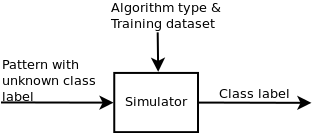
\includegraphics{fig/schema.png}
    \end{center}
    \caption{General schema of simulation environment. Input/output of the
    system}
    \label{fig:input_output}
\end{figure}

\subsection{Scope of this project} 
This paper comprises of two parts. In the first, the review of
literature and the basic notation used in the whole thesis is presented. Section
\ref{cha:Introduction} is the source of the basic
knowledge about pattern recognition. Sections \ref{cha:Rough_set}, \ref{cha:Fuzzy_logic}
present the description of algorithms used in this thesis. Additionally, this
part shows algorithm construction steps using pseudo-code.

The second part, which is the main point of this thesis, presents experiments analysis.
Paragraph \ref{cha:ExperimentAnalysis} describes the experiment environment
setting and program written in \textit{Python} to simulate all implemented
algorithms.  Results with comments are placed in
section \ref{cha:Simulation_investugations}. General
conclusions and plans for the future work are placed in sections
\ref{cha:Summary}, \ref{cha:FutureWork}, respectively. 



%\section{Problem statement}
Genetic algorithms can be computationally expensive as the result of
complexity within particular application or due to the sheer numbers needed to
reach an acceptable solution. In many problems found in the literature the
expense of a genetic algorithm is due to both these factors \cite{bib5},
\cite{bib7}, \cite{bib11}. The genetic algorithm is a global searching process
based on Darwin's principle of natural selection and evolution, so taking into
account this fact many scientists have noticed that program simulating genetic
algorithms can be implemented in various ways, from
simple sequential program to different method of parallelization. The advent of
multiprocessors has spawned a number of $\mathcal{GA}$ implementations which take advantage
of parallelism available in the algorithm(migration process, subpopulations,
diffusion) \cite{bib8}, \cite{bib9}. In recent years, multi-population genetic algorithms $\mathcal{MGA}$ 
have been recognized as being more effective both in speed and solution quality 
than single-population genetic algorithms $\mathcal{SGA}$. Despite of these advantages,
the behavior and performance of $\mathcal{MGA}$ is still heavily 
affected by a~judicious choice of parameters, such as connection topology, 
migration method, migration interval, migration rate, population number and many
others. The main problem in this topic is to find the best topology, configuration
parameters and balance between the potential speedup and number of slaves.


\section{Pattern recognition algorithms}
\label{cha:Introduction}
\subsection{Introduction}
This section is devoted for presenting information about pattern recognition
algorithms. The main purpose is to describe algorithms that are used in this
thesis. 

Pattern recognition is a wide area of science in which we are interested in
assigning label from a given set of classes to every unknown pattern. The whole 
process of classification can be divided into few phases, where each has a
significant impact on the final classification accuracy:
\begin{enumerate}
    \item Data collection
    \item Feature selection
    \item Model selection
    \item Classifier selection
    \item Training 
    \item Testing
\end{enumerate}
At first in this section few basic information and categories will be given 
about pattern recognition. Generally, the whole process of classification
can be broken down into two main categories:
\begin{itemize}
    \item supervised - incoming to the system objects are not previously
        labeled and this is the system task to find an appropriate structure of
        the data, to establish the organization of the classes basing only on
        the available data, there is no statistical or expert knowledge at a
        hand.
    \item unsupervised - in this approach incoming patterns have labels and can
        be treated as a training set. This allows the classifier can retrieve
        information from data 
\end{itemize}
In this thesis supervised learning is reconsidered because available datasets 
are labeled with class number. Further division is connected with syntactic and statistical 
approach. In former, each pattern is represented in terms of 
$d$ features (measurements) and is viewed as a point in
$d$-dimensional feature space, while the latter
is based on the characterization of the inherent structure of the 
qualitative features. For that  reason, the complex patterns can be
decomposed using a hierarchical structure in simple  sub-patterns.
The patterns are viewed as sentences belonging to a language, primitives
represents the alphabet of the language and the sentences are generated
according to a grammar which is inferred from the available training data.
EKG waveforms, textured images and shape analysis of contours are the examples
of syntactic approach.

\subsection{Problem statement for pattern recognition task}
\label{cha:Problem_statement}
In this section the problem statement will be presented in case of pattern
recognition algorithm. For the purpose of this thesis we assume a supervised learning and
denote each pattern by the label $j \in M$, where $M$ is an $m$-element set of
possible states numbered with the successive natural numbers. The state $j$ is
unknown and does not undergo the direct investigation. What can only be
measured are attributes or features by which a state manifests itself. For this
reason each object(pattern) will be described by a $d$-dimensional measured feature vector $x \in
X$. In order to classify unknown pattern algorthm uses knowledge stored in the training
set consisting of $N$ training patterns:
\begin{equation}
    S = (x_1, j_1), (x_2, j_2), \ldots, (x_N, j_N)
    \label{eq:training_pattern}
\end{equation}
In practice the decision algorithm  with learning phase should use knowledge included in the
training set $S$ and as the consequence the algorithm with learning is of the
following form:
\begin{equation}
    i=\Psi(S, x), \, i \in M
    \label{eq:decision_algorithm}
\end{equation}
In decision theory, to ensure that $\Psi$ approximates the problem as closely
as possible an additional loss function is introduced that assigns a specific
value to the loss resulting from producing an incorrect label. The particular loss
function depends on the type of label being predicted. In case of
classification problem it is zero-one loss function. This corresponds simply to
assigning a loss value of 1 to any incorrect labeling and is equivalent to computing
the accuracy of classification procedure over the set of training data.

\subsection{Rough sets}
\label{cha:Rough_set}
\subsubsection{Introduction}
\label{cha:Rough_set_introduction}
Rough sets theory represents the mathematical approach to deal with imperfect knowledge. 
In the standard standard pattern recognition task we need precise information about pattern to recognize, 
while rough sets can deal with vague or incomplete data. The problem of imperfect 
information has been tackled for a long time and it has become a crucial issue for many scientist.
One of the most prominent approaches in the recent years are fuzzy logic and rough sets.
In this section the latter approach is presented in greater details. 

Comparing with other methods, rough sets have many advantages, but one of the most important
one is its ability to works only on the raw data, with no additional information such 
as density probability in Bayesian algorithm \cite{bib38}, \cite{bib14}. The main facts about rough sets
algorithm can be summarized in few point presented below:
\begin{enumerate}
    \item simplifies data by the granulation pre-processing
    \item is able to reduce attributes
    \item generates set of easy to understand and readable decision
        \textit{IF-THEN} rules
    \item evaluates significance of data 
\end{enumerate}

When talking about rough set theory one has to understand the concept of a set 
and how a rough set is related to the classical set represented in mathematic.
From the mathematical point of view the crisp (precise) set is a collection of 
objects of interest and is uniquely determined by its elements. In other words,
it means that every element must be uniquely classified as belonging to the set 
or not (true or false). For example, the set of odd numbers is crisp because every
number is either odd or even and cannot be partially in both. 

Generally, we come across problem form the nature that are much more
complicated than simple decision whether an objects belong to the set or not. 
For some sets we cannot precisely describe element
membership. Reconsider the group of people and division into set of small and
high people. The height is not a precise but a vague concept and data vagueness can 
be met in many problems found in the nature. Here is the spot for rough sets
theory where vagueness is expressed by a boundary region of a set. 

\subsubsection{Basic notation}
\label{cha:Rough_set_basic_notation}
In rough sets theory to represent datasets (information) we introduce a notion 
called an \textit{information system} \cite{bib37}, \cite{bib39}. 
It can be described by 4-tuple
\begin{equation}
    IS = <U, Q, V, f >
    \label{eq:information_system}
\end{equation}
where the notation used in eq. (\ref{eq:information_system}) is as follows:
\begin{itemize}
    \item $U$ is the universe of discourse  which is a finite set of objects
        (patterns)
    \item $Q$ is a finite set of attribute by  which each patterns manifests
        itself (is described)
    \item $V = \bigcup V_q$, $V_q$ represents a domain of attribute $q$
    \item $f:U \times Q \rightarrow V$ is a total information function, such that
        $\bigvee_{q\in Q, x \in U} f(x,q) \in U$
\end{itemize} 
The information system can be represented as a finite table in which 
columns are labeled by attributes and each rows stands for an object from
$IS$. Over the information table we can define decision table
$T$ where the set of attributes $Q$ is disjoined into two
subset $C$ and $D$. The set $C$ is a subset of 
condition attributes, and the set $D$ contains decision attributes 
by which we can partition set $U$ into decision classes.

From the granular nature of rough sets it may happen that some objects 
in the $U$ are indistinguishable due to the limited information caused by
granulation process. Taking this into account let define an indiscernibility
relation $R \rightarrow U \times U$, representing the 
lack of knowledge about patterns in the set $U$. The indiscernibility relation on
$U$ can be extended and associated with every non-empty subset of attributes $P \subseteq Q$
and is defined by eq. (\ref{eq:indiscernibility})
\begin{equation}
    I_P = \{ (x, y) \in U \times U: f(x, q) = f(y,q), \bigvee_{q \in P}\}
    \label{eq:indiscernibility}
\end{equation}
Now having $I_P$ we can say that objects $x$ and
$y$ are $P$-indiscernible by a set of attributes $P$ if $y \, I_P \, x$. Relation
$I_P$ divides the set $U$ into blocks (concepts) of $P$-indiscernible objects.
The $P$-elementary set containing objects $P$-indiscernible with $x \in U$ is
referred as $I_P(x)$ and defined as follows:
\begin{equation}
    I_P = \left\{ y \in U: y \, I_P \, x \right\}
    \label{eq:p_indiscernible}
\end{equation}

By representing a target concept $X$ as a subset of $U$ we would like to
describe it with respect to $R$. Additionally let assume $P$ as non-empty
subset of attributes from $Q$. In rough sets reasoning an object membership to a
set can be represented in two ways:
\begin{enumerate}
    \item An object $x \in U$ certainly belongs to $X$ if
        all objects from the $P$-elementary set defined by $I_P(x)$ also belong to $X$.
        A set of all objects certainly belonging to $X$ creates the $P$-lower
        approximation of $X$ and can be represented as follows:
        \begin{equation}
            \underline{I_P} = \{ x \in U: I_P(x) \subseteq X\}
            \label{eq:lower_approximation}
        \end{equation}
    \item An object $x \in U$ can possibly belong to $X$ if at least one object
        from $P$-elementary set $I_P(x)$ can possibly belong to $X$. All the
        objects that could possibly belong to $X$ are denoted as $P$-upper
        approximation of $X$, defined as:
        \begin{equation}
            \overline{I_P} = \{x\in U: I_P(x) \, \cap \, X \neq \emptyset \}
            \label{eq:upper_approximation}
        \end{equation}
        Therefore the set $U - \overline{I_P}$ represents the negative region
        containing the set of objects that can be definitely ruled out as
        members of the target set $X$.
\end{enumerate}

The tuple $<\underline{I_P}, \overline{I_P}>$ representing a lower boundary of
the target $X$ and the upper boundary of the target $X$ creates a rough set \cite{bib34}.
Using above notion we can define $P$-boundary region which is a difference
between upper and lower approximation \cite{bib14}. 
\begin{equation}
    BN_P(X) = \overline{I_P} - \underline{I_P}
    \label{eq:boundary_region}
\end{equation}
The $BN_P(X)$ is a set of elements which cannot be certainly classified neither
as $X$ nor as not-$X$ with respect to the set of attributes $P$. If the
boundary region of $X$ is empty then the set represented by tuple
$<\underline{I_P}, \overline{I_P}>$ 
is crisp, otherwise we deal with inexact set which is called rough set. 
Until this moment we can see that rough sets concept can be defined quite generally by means of topological
operations: interior and closure, called approximations. They express the
knowledge about pattern in terms of granules, not by a precise measure
\cite{bib40}.

The illustrative example of rough sets reasoning is presented in fig. \ref{fig:rough_set_example}
\begin{figure}[H] 
    \begin{center}
        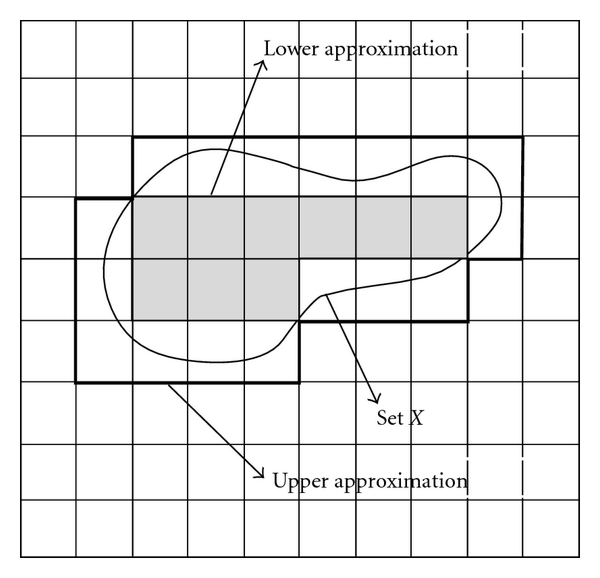
\includegraphics{fig/rough_set.png}
    \end{center}
    \caption{Rough sets example presenting lower and upper approximations}
    \label{fig:rough_set_example}
\end{figure}

\subsubsection{Rough sets indicators}
\label{cha:Rough_sets_indicators}
In rough sets theory we can define few indicators. First of all with every 
subset of $X \subseteq U$ described by $P$ subset of attributes we can 
associate an indicator called an accuracy of approximation defined as:
\begin{equation}
    \alpha_P(X)=\frac{\underline{I_P}(X)}{\overline{I_P}(X)}
    \label{eq:accuracy_approximation}
\end{equation}
The grater $\alpha_P(X)$ is, the better approximation we have which means that
many objects can be certainly classified as belonging to the target set $X$.

Another important indicator is a quality of approximation of $X \subseteq U$ by
attributes from subset $P$. It represents the percentage of correctly classified 
objects using attributes $P$ from subset $X$:
\begin{equation}
    \gamma_P(X) = \frac{\overline{I_P}(X)}{|X|}
    \label{eq:quality_approximation}
\end{equation}
Assuming that we can partition $U$ into $n$ decision classes using $P$
non-empty subset of attributes from $C$, the quality of classification can be
defined as the ration of all correctly classified objects into classes:
\begin{equation}
    \gamma_P(CLASS) = \frac{\sum_{i=1}^{n}\overline{I_P}(CL_i)}{|U|}
    \label{eq:class_quality}
\end{equation}

These indicators can be used in determining the quality of rough set algorithm
or for finding the optimal reduct. Generally, the main goal in constructing
rough sets algorithm is to obtain rule set with possible the greatest number of
certain decisions.

\subsubsection{Properties of rough sets}
The same as classical sets, rough sets can be described by the
following properties:
\begin{enumerate}
    \item $\overline{I_P} \subseteq \, X \, \subseteq \, \underline{I_P}$
    \item $\overline{I_P}(\emptyset) = \underline{I_P}(\emptyset) = \emptyset;
        \;
        \overline{I_P}(U) = \underline{I_P}(U) = U $
    \item $\overline{I_P}(X \cup Y) = \overline{I_P}(X) \cup \overline{I_P}(Y)$
    \item $\underline{I_P}(X \cap Y) = \underline{I_P}(X) \cap \underline{I_P}(Y)$
    \item $\overline{I_P}(U-X) = -\underline{I_P}(X)$
    \item $\underline{I_P}(U-X) = -\overline{I_P}(X)$
\end{enumerate}
It is easily seen that the lower and the upper 
approximations of a set are interior and 
closure operations in a topology generated by the 
indiscernibility relation $I_P(X)$. Additionally, in rough sets theory 
we can define four types of data vagueness \cite{bib40}:
\begin{itemize}
    \item $\overline{I_P}(X) \neq \emptyset,\, \underline{I_P}(X) \neq
        \emptyset$ $IF\; X$ is roughly $I_P$-definable. It means that for some
        elements from $U$ we can decide whether they belong to $X$ or $U-X$
        using $I_P$
    \item $\overline{I_P}(X) \neq \emptyset,\, \underline{I_P}(X) \neq U$ $IF\;
        X$ is internally $I_P$-indefinable. It means that we are able to decide
        which elements from $U$ belong to $U-X$, but we don't know if they
        belong to $X$ using $I_P$
    \item $\overline{I_P}(X) \neq \emptyset,\, \overline{I_P}(X) = U$ $IF\;
        X$ is externally $I_P$-definable. It means that we are able to decide
        which elements from $U$ belong to $X$, but we don't know if they belong
        to $U-X$ using $I_P$
    \item $\overline{I_P}(X) \neq \emptyset,\, \overline{I_P}(X) = U$ $IF\;
        X$ is totally $I_P$-indefinable. It means that we are unable to decide
        for any element from $U$ if it belongs to $X$ or $-X$ using $I_P$
\end{itemize}
\subsubsection{Rough sets reasoning from data}
The category description can be done in two ways:
\begin{enumerate}
    \item extensional
    \item intentional
\end{enumerate}
Each of these approaches differs in the way how pattern from dataset is
represented. To represent a concept we have to be able to identify all objects belonging 
to this category. With the former approach we have no insight 
into decision engine so we do not know how to assign new objects to the category.
In the latter approach we represent the category based on the set of rules. The same 
approach is done in rough sets algorithm where an elementary 
granules (concepts) of knowledge build blocks consisting 
of indiscernible pattern from the universe of discourse $U$. 
As stated in section \ref{cha:Rough_set_basic_notation} reconsidered dataset or
problem can be represented as a table. When decision attributes from $D$ are
added to the table it is transformed into decision table $T$ where each
row is associated with decision rule.

In this section a practical example will be presented to clear all the things
out. As an example let reconsider well-known problem of patients suffering from
flu \cite{bib39}, \cite{bib40}. The task is to decide if a patient described by 3 attributes is ill or not. Table \ref{tab:example_rough_set} 
represents an information system $IS$ about healthy patient and those suffering
from flu. Attributes: \textit{Headache}, \textit{Muscle-pain},
\textit{Temperature} are called condition attributes and denoted as ($c_i,i \in (1, \ldots, q)$),
while the attribute \textit{Flu} (last column in table \ref{tab:example_rough_set}) is considered as
a decision attribute $c_d$.
\begin{table}[H] 
    \centering
    \caption{Example dataset showing healthy patients and suffering from flu}
    \begin{tabular}{|c|c|c|c|c|c|}
        \hline 
    Patient & Headache $c_1$& Muscle pain $c_2$& Temperature $c_3$& Flu $c_d$\\ \hline \hline
    p1 & no & yes & high & yes \\ \hline
    p2 & yes & no & high & yes \\ \hline
    p3 & yes & yes & very high & yes \\ \hline
    p4 & no & yes & normal & no \\ \hline
    p5 & yes & no & high & no \\ \hline
    p6 & no & yes & very high & yes \\ \hline    
    \end{tabular}
    \label{tab:example_rough_set}
\end{table}
Each row of a decision table determines a decision rule. 


\begin{tabular}[H]{l}
    Rule 1:  IF $c_1$ IS 'NO' AND $c_2$ IS 'YES' AND $c_3$ IS 'HIGH' THEN $c_d$
    IS 'YES' \\
    Rule 2:  IF $c_1$ IS 'YES' AND $c_2$ IS 'NO' AND $c_3$ IS 'HIGH' THEN $c_d$
    IS 'YES' \\
    Rule 3:  IF $c_1$ IS 'YES' AND $c_2$ IS 'YES' AND $c_3$ IS 'VERY HIGH' THEN
    $c_d$ IS 'YES' \\
    Rule 4:  IF $c_1$ IS 'NO' AND $c_2$ IS 'YES' AND $c_3$ IS 'NORMAL' THEN
    $c_d$ IS 'NO' \\
    Rule 5:  IF $c_1$ IS 'YES' AND $c_2$ IS 'NO' AND $c_3$ IS 'HIGH' THEN $c_d$
    IS 'NO' \\
    Rule 6:  IF $c_1$ IS 'NO' AND $c_2$ YES 'NO' AND $c_3$ IS 'VERY HIGH' THEN
    $c_d$ IS 'YES'  
\end{tabular}


After analyzing table \ref{tab:example_rough_set} it is noticeable that some
patients cannot be distinguished between each other, for example $p2$ and $p5$.
It is possible to generate different indiscernible relations based on 
the chosen attributes. In case of \textit{Headache} attribute patients: $p2$,
$p3$, $p5$ are indiscernible; patients $p2$, $p5$ are
indiscernible with respect to attributes \textit{Headache},
\textit{Muscle-pain} and \textit{Temperature}, or if we use \textit{Headache}
and \textit{Muscle-Pain} the set $U$ can be divided into three sets:
\{$p1$, $p4$, $p6$\}, \{$p2$, $p5$\}, \{$p3$\}.

Now it is time for defining key features of rough sets. Over the table
\ref{tab:example_rough_set} we can define two concepts (target sets):
\textit{Flu} and \textit{Not Flu}. For the first concept the lower approximation
set of patient certainly having flu is \{$p1$, $p3$, $p6$\}, while the upper
approximation of patients possibly suffering from flu is \{$p1$, $p2$, $p3$,
$p5$, $p6$\}. The boundary region for concept \textit{Flu} is a set of \{$p2$, $p5$\} 
patients. For the concept \textit{Not Flu} the lower approximation is the set
\{$p4$\}, whereas the upper approximation is the set \{$p2$, $p4$, $p5$\}. Again the 
boundary region is the set \{$p2$, $p5$\}.

Additionally, we can measure the accuracy of approximation $\alpha_P(x)$ for each concept.
This can indicate if the set of attributes used for describing the concept is correctly
chosen. For the \textit{Flu} concept where $X$=\{$p1$, $p2$, $p3$, $p6$\} is described by
set of attributes $P$=\{\textit{Headache}, \textit{Muscle-pain},
\textit{Temperature}\} the accuracy of approximation is:
$$\alpha_P(Flu) = \frac{3}{5}$$
On the other hand when we take only one attribute $P$=\{\textit{Temperature}\}, then we get lower approximation of 
\{$p3$, $p6$\} and upper approximation of \{$p1$, $p2$, $p3$, $p5$, $p6$ \}
resulting in:
$$\alpha_P(Flu) = \frac{2}{5}$$
To sum up, $\alpha_P(x)$ is a very important indicator in
rough sets theory and tells which attributes better characterize target
concept. This example has shown that because of the granule representation of
knowledge in rough sets approach some object cannot be discerned. It is very
important to choose proper condition attributes because this determines how
upper and lower approximations are represented by objects from $U$. 


\subsection{Fuzzy logic}
\label{cha:Fuzzy_logic}
\subsubsection{Introduction}
In fuzzy logic an element membership to a set is described by a membership function 
which assigns value from interval $[0, 1]$:
\begin{equation}
    \mu_A:U\rightarrow [0,1], \, A \subseteq U
    \label{eq:fuzzy_function}
\end{equation}
The properties of membership function $\mu$ are as follows:
\begin{itemize}
    \item $\mu_{\emptyset}(x) = 0, \, x \in U$
    \item  $\mu_{U}(x) = 1, \, x \in U$
    \item  $\mu_{X}(x) \leq \mu_{Y}(x), \, IF X \subseteq Y$
    \item  $\mu_{\overline{A}}(x) = 1 - \mu_{A}(x), \, x \in U$
\end{itemize}
where $\emptyset$ is an empty set and $\overline{A}$ is the complement of the
set $A$.

Fuzzy logic is a superset of Boolean logic that 
has been extended to handle the concept of partial truth - values between ``completely 
true'' and ``completely false'' \cite{bib6}, \cite{bib12}. This theory was introduced by 
Dr. Lotfi Zadeh in the 1960's as a tool for modelling the uncertainty of natural language. 
This approach can be applied to many problems, analyze only few examples:
\begin{itemize}
    \item Days of a week- there is a question which day is mostly associated
        with a weekend. Generally, we would assume that the membership value
        $g$ associated with each day will be as follows:
        \{Monday=0, Tuesday=0.2, Wednesday=0.4, Thursday=0.5, Friday=0.7,
        Saturday=1.0, Sunday=0.9\}
    \item The seasons- there is not evident boundary when one season stops and
        another starts. This example can be illustrated quite precisely by fig.
        \ref{fig:seasons}.
        \begin{figure}[H]
            \begin{center}
                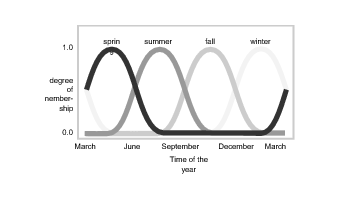
\includegraphics{fig/seasons.png}
            \end{center}
            \caption{Example of how fuzzy logic can be used to describe the
            season of the year}
            \label{fig:seasons}
        \end{figure}
    \item The height: small and tall definitions- from the group of people it
        is hard to define who is tall and who is small interchangeably. To
        solve this problem we can define the concept \textit{Tall} and assign
        value to each person describing its value. This process is presented in
        fig. \ref{fig:fuzzy_tall}
        \begin{figure}[H]
            \begin{center}
                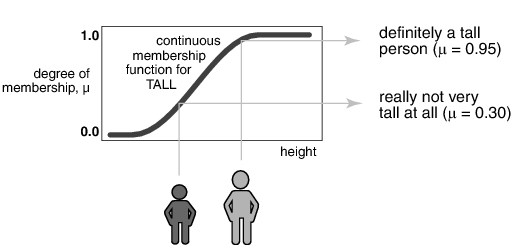
\includegraphics{fig/fuzzy_tall.png}
            \end{center}
            \caption{Fuzzy approach for defining person height}
            \label{fig:fuzzy_tall}
        \end{figure}
\end{itemize}

As in the section \ref{cha:Rough_set_introduction}, let reconsider the problem of defining 
if person is small or tall more deeply. First of all, we have to define a fuzzy
set (concept) \textit{Tall} which will answer the question 
"to what degree is person x tall?". Zadeh describes \textit{Tall} as a
linguistic variable, which represents our cognitive category of "tallness"
\cite{bib25}. To each person in the universe of discourse, 
we have to assign a degree of membership in the fuzzy subset \textit{Tall}
based on the membership function (for example the same as presented in fig.
\ref{fig:fuzzy_tall}). Table \ref{tab:fuzzy_logic_example} shows an example of fuzzy
reasoning:
\begin{table}[H]
    \centering
    \caption{Table describing how person is tall by the fuzzy logic linguistic
    variable}
    \begin{tabular}{|c|c|c|}
        \hline
        Person & Height [m] & degree of tallness \\ \hline \hline
        p1 & 1.5 & 0.0 \\ \hline
        p2 & 1.6 & 0.2 \\ \hline
        p3 & 1.7 & 0.4 \\ \hline
        p4 & 1.8 & 0.5 \\ \hline
        p5 & 1.9 & 0.6 \\ \hline
        p6 & 2.0 & 1.0 \\ \hline
    \end{tabular}
    \label{tab:fuzzy_logic_example}
\end{table}

Fuzzy numbers are fuzzy subsets generated over the attribute domain. 
They have a peak or plateau with membership grade 1, over which the 
members of the universe are completely in the set.  The membership 
function is increasing towards the peak and decreasing away from it. 
There are different types of membership functions and their usage 
strongly depends on the type of reconsidered problem. One of the most 
commonly used in the literature are: triangular, trapezoidal, Gaussian shapes
(see example in fig. \ref{fig:fuzzy_example_1}).

\subsubsection{Fuzzy reasoning from data}
Reasoning in fuzzy logic is based on decision rules the same as in rough sets
approach \cite{bib11}. 
Rules are expressed in the form of IF \textit{COND} THEN \textit{DECISION} 
which can be divided into antecedent set ($A_{ri}, \, i \in (1, \ldots, q)$) and one consequent determining the
output of the rule. In the pattern recognition task when we deal with patterns
described by $d$ features rules have the form presented by eq. (\ref{eq:rule_example})
\begin{equation}
    IF\, x_1=A_{r1}\, AND\, x_2=A_{r2}\, AND\, \ldots\, AND\, x_d=A_{rd}\, THEN\,
class\, C_r\, with \, CF_r
    \label{eq:rule_example}
\end{equation}

The \textit{AND}, \textit{OR}, and \textit{NOT} operators of 
Boolean logic exist in fuzzy logic and are usually defined as the minimum, maximum,
and complement. When they are defined this way, they are called the Zadeh
operators \cite{bib2}.

Fuzzy logic classification is based on three main steps:
\begin{enumerate}
    \item Fuzzyfication- in the fuzzyfication process we 
        convert continuous quantity into fuzzy number based on the appropriate
        membership function value. It requires defining
        membership grade of crisp input $x$ in the fuzzy set.
    \item Rule induction- there are different types of fuzzy inference systems,
        but one of the most commonly used (the same as in this paper) is
        Mamdani inference system \cite{bib46}.
    \item Deffuzification- the process of producing a quantifiable result in
        fuzzy logic from given fuzzy sets and corresponding membership degrees. 
\end{enumerate}
The whole process of fuzzy reasoning is presented in fig.
\ref{fig:fuzzy_reasoning}
\begin{figure}[H]
    \begin{center}
        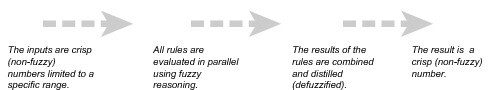
\includegraphics[width=\textwidth]{fig/fuzzy_steps.png}
    \end{center}
    \caption{Steps applied in fuzzy reasoning.}
    \label{fig:fuzzy_reasoning}
\end{figure}

Let reconsider a simple example, which should clear all ambiguities (the following 
example is based on \cite{bib0}). The problem is connected with estimating the
level of risk involved in software engineering project. There are two input
to the system (funding, staffing) and one output
(risk). Membership functions are represented as triangular shapes (fig. \ref{fig:fuzzy_example_1}) 
\begin{figure}[H]
    \begin{center}
        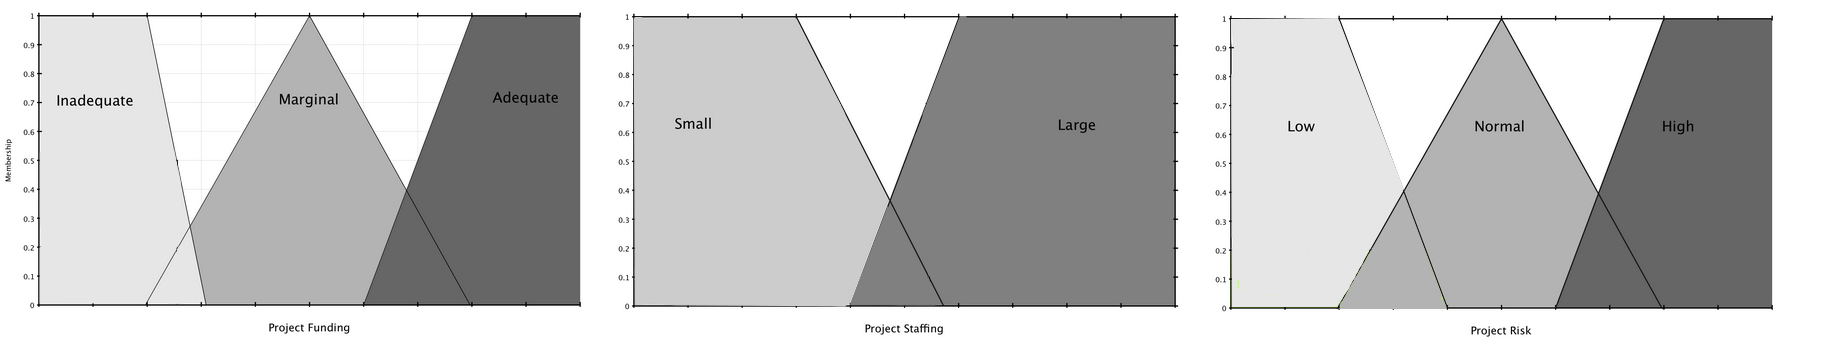
\includegraphics[width=\textwidth]{fig/fuzzy_example_1.png}
    \end{center}
    \caption{Input and output fuzzy linguistic variables for the described
    system.}
    \label{fig:fuzzy_example_1}
\end{figure}
The next important thing in fuzzy logic beside fuzzy values are fuzzy rules. In
this problem they are provide a priori and are in the following way:
\begin{table}[H]
    Rule 1: IF funding IS adequate OR funding IS small THEN risk IS
    low \\
    Rule 2: IF funding IS marginal AND staffing IS large THEN risk IS
    normal \\
    Rule 3: IF funding IS inadequate THEN risk IS high
\end{table}
Let say that we want to calculate project risk for inputs: funding~$=35$ and
staffing~$=60$. 
\begin{enumerate}
    \item The first step is to convert crisp values into fuzzy representation.
        Activating each input membership functions fuzzy values are as follows:
        $$
            \begin{array}[H]{l}
                input \;1 \\ \hline
                \mu_{inadequate}(35) = 0.5 \\
                \mu_{marginal}(35) = 0.2 \\
                \mu_{adequate}(35) = 0.0 \\ \\
                input 2 \\ \hline
                \mu_{small}(60) = 0.1 \\
                \mu_{large}(60) = 0.7 \\ 
            \end{array}
        $$
    \item Now it is time f or rule induction where OR is treated as a $max$ operator, AND
        as $min$ operator. 
        $$
            \begin{array}[H]{ll}
                Rule \,1: & \mu_{low} = 0.0 + 0.1 = 0.1 \\
                Rule \,2: & \mu_{normal} = 0.2\cdot 0.7 = 0.14 \\
                Rule \,3: & \mu_{high} = 0.5 \\
            \end{array}
        $$
    \item After performing clipping of consequent membership functions for each
        rule (example given in fig. \ref{fig:fuzzy_centroid}), the final crisp output can be calculated. It is done by
        defuzzification method, where one of the most commonly used is a centroid
        formula given by eq. (\ref{eq:fuzzy_centroid}) \cite{bib0}, \cite{bib1}.
        \begin{equation}
            CO = \frac{\sum\nolimits_{x=a}^{b}\mu_A(\chi)\cdot
            x}{\sum\nolimit_{x=a}^{b}\mu_A(\chi)}
            \label{eq:fuzzy_centroid}
        \end{equation}
        \begin{figure}[H]
            \begin{center}
                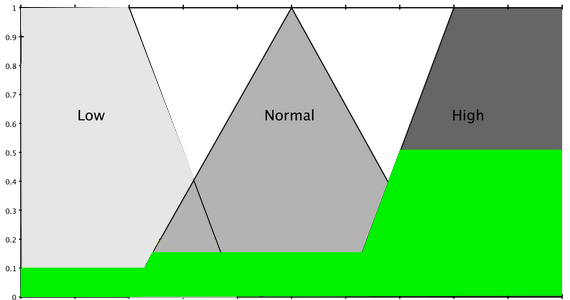
\includegraphics[width=0.6\textwidth, height=0.4\textwidth]{fig/fuzzy_centroid.png}
            \end{center}
            \caption{Example of clipping the consequent membership function
            as the result of rule induction}
            \label{fig:fuzzy_centroid}
        \end{figure}
        Using eq. (\ref{eq:fuzzy_centroid}) the output of the system is as follows:
        $$
        CO = \frac{(0+10+20)\cdot 0.1 + (30+40+50+60)\cdot 0.14 + (70 + 80 + 90
        + 100)\cdot 0.5}{0.1\cdot 3 + 0.14\cdot 4 + 0.5\cdot 4 } = 69.3
        $$
    It means that for input values funding~$=35$ and staffing~$=60$ the project
    risk is about $69\%$.
\end{enumerate}
\subsubsection{Genetic-based machine learning approaches}
In the literature one can find many examples of fuzzy logic applications
\cite{bib3}, \cite{bib9}.
Generally, there are two main approaches:
\begin{enumerate}
    \item some expert knowledge is available and fuzzy rules are created
        beforehand.
    \item no knowledge about data set is present so some techniques of data
        mining must be applied to extract rules from the training set.
\end{enumerate}
At this point it must be strongly emphasized that in this thesis the main focus is based on
fuzzy algorithm for pattern recognition task where there is no prior knowledge 
about fuzzy system and decision rules. There are different approaches for
construction fuzzy logic algorithm from raw dataset, for example optimization techniques
such as gradient descent or heuristic algorithms \cite{bib8}, \cite{bib16},
\cite{bib28}. In this paper the genetic algorithm
is proposed for creating an optimal rule set. 

One can wonder what is the purpose of applying genetic algorithm into rule
generation. For the simplicity let reconsider such a case. $N$ training
patterns are available and nothing more. Now the following question arises: 
how to properly divide the feature space into fuzzy set, and how to generate
decision rules when there is no expert knowledge. The simplest and
straightforward solution is to create let say 10 triangular membership functions for each
attribute, and check each possible combination. Is this approach optimal? The
efficiency of this solution strongly depends on the complexity of the problem.
For $d$-dimensional feature space and $k$ fuzzy membership function per each attribute
the number of possible combination for generating one rule is equal to $k^d$.
For greater $d$ (for example wine dataset from \textit{UCI} repository has 13
attributes) it is impossible to find the proper combination in a reasonable
time. Here is an open spot for genetic algorithm to show its searching
abilities.

There are two main methods of genetic-based machine learning approaches
\cite{bib30}, \cite{bib31}:
\begin{enumerate}
    \item Michigan template- it is a population of fuzzy rules and a single
        fuzzy rule is handled as an individual (see fig. \ref{fig:michigan}). 
        The evaluation of each fuzzy rule is performed by classifying all the 
        given training patterns by the available rule set $N_{rule}$. At the 
        end of each iteration new individuals are created through genetic operators 
        and merged to the current population. For the next generation $N_{rule}$ 
        best individuals are taken. The whole procedure can be summarized as follows:
        \begin{enumerate}
            \item Generate $N_{rule}$ fuzzy rules
            \item Evaluate the fitness of each fuzzy rule in the current
                population
            \item Generate $N_{replace}$ fuzzy rules using genetic operators
            \item Merge $N_{replace}$ fuzzy rules with current population and
                choose the best $N_{rule}$ individuals for the next generation
            \item Return to point $(b)$ is stopping condition is not fulfilled
                (number of generations)
        \end{enumerate}
        \begin{figure}[H]
            \begin{center}
                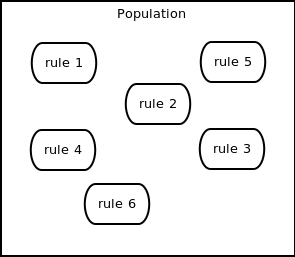
\includegraphics[width=0.5\textwidth, height=0.4\textwidth]{fig/michigan.png}
            \end{center}
            \caption{Example of Michigan approach for constructing Genetic
            Fuzzy logic algorithm}
            \label{fig:michigan}
        \end{figure}
    \item Pittsburgh template- in this approach a set of fuzzy rules is handled
        as an individual (see fig. \ref{fig:p}). In this case the length of a single individual is
        equal to $n\cdot N_{rule}$, where $n$ is the length of single fuzzy rule.
        Algorithm starts with $N_{pop}$ randomly generated rule sets. The
        fitness value of a single individual is the number of correctly
        classified patterns in the training set by a given rule set.
        The procedure for algorithm is as follows:
        \begin{enumerate}
            \item Generate $N_{pop}$ individuals consisting of $N_{rule}$ fuzzy
                rules each
            \item Calculate the fitness value of each rule set (individual)
            \item Generate $N_{replace}$ new rule set using genetic operators.  
            \item Merge $N_{replace}$ fuzzy rule sets  with current population and
                choose the best $N_{pop}$ individuals for the next generation
            \item Return to point $(b)$ is stopping condition is not fulfilled
                (number of generations)
        \end{enumerate}
        \begin{figure}[H]
            \begin{center}
                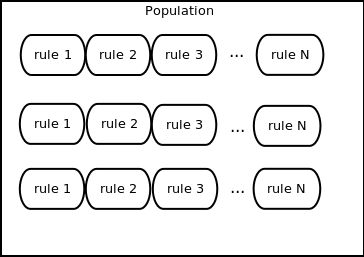
\includegraphics[width=0.5\textwidth, height=0.4\textwidth]{fig/pittsburgh.png}
            \end{center}
            \caption{Example of Pittsburgh approach for constructing Genetic
            Fuzzy logic algorithm}}
            \label{fig:p}
        \end{figure}
\end{enumerate}
In this thesis the first approach will be implemented which means that
individual is modelled as a single rule. 

\subsection{Attribute reduction}
\label{cha:Attribute_reduction}
Many problem are complex and multidimensional. For example Sonar dataset from
\textit{UCI} Repository has 60 attributes describing a single pattern. 
Usually we hope to recognize pattern in a relatively
lower dimensional to reduce cost in measuring and processing information and
enhance the interpretability of learned models. Feature selection or reduction 
is done for classifiers to remove the noise and superfluous data. Generally,
this is not an easy task and requires a lot of computation \cite{bib1}, \cite{bib5}.  

A reduct is a set of attributes that ensures the same classification of
elements from $U$ as the rudimentary set of attributes. More than one reduct
can exist for one information system. The core of attributes is the set of
attributes from $Q$ that all the attributes are indispensable. An attribute is
dispensable if the following criterion is fulfilled:
$$I(P) = I(P-{a}), \, \textrm{for} \, \{a\} \in P \subseteq  Q $$

In the literature there are many examples of how to apply attribute reduction
\begin{itemize}
    \item information measures
    \item distance measures
    \item dependence measures
    \item consistency measures
\end{itemize}
Different approaches provide various results and their application strictly
depend on the type of data. One of the best known methods are Principal
Component Analysis, Factor analysis or optimization and heuristic techniques.
In the recent years heuristic techniques are very often used because of their
speed and searching abilities. A lot of work has been devoted for feature
extraction and this is not the intention to explore this area of research.
Basing on the results conclusions presented in the literature, in this thesis a 
genetic algorithm is proposed for extracting valuable features from the set of 
all attributes \cite{bib27}, \cite{bib48}.

\subsection{Genetic algorithm}
\label{cha:Genetic_algorithm}
Genetic Algorithm is an element of evolutionary computation, which is a 
rapidly growing area of soft computing \cite{bib42}, \cite{bib43}. GA is based on the principles of
natural selection and genetic modification. As optimization methods, GA 
operates on a population of points, designated as individuals. Each 
individual of the population represents a possible solution of the 
optimization problem. Individuals are evaluated depending upon their 
fitness which indicates how well an individual of the population solves 
the optimization problem. To sum up, GA has the following general features:
\begin{enumerate}
    \item GA operates with a population of possible solutions (individuals) 
        instead of a single individual. Thus, the searching process can be 
        carried out in a parallel form or sequentially.
    \item GA is able to find the optimal or sub-optimal solutions in complex
        and large search spaces. Moreover, it can be applied to nonlinear 
        optimization problems with constraints defined in discrete or continuous 
        search spaces.
    \item GA examines many possible solutions at the same time, so there is a 
        higher probability that the search process can converge to an optimal solution.
\end{enumerate}
There are four main parts in each GA process to reconsider (graphically
presented as a flow chart \ref{fig:genetic_scheme}):
\begin{enumerate}
    \item the problem representation or encoding
    \item fitness or objective function definition
    \item fitness-based selection
    \item evolutionary reproduction of candidate solutions (individuals or chromosomes). 
\end{enumerate}
\begin{figure}[H]
    \begin{center}
        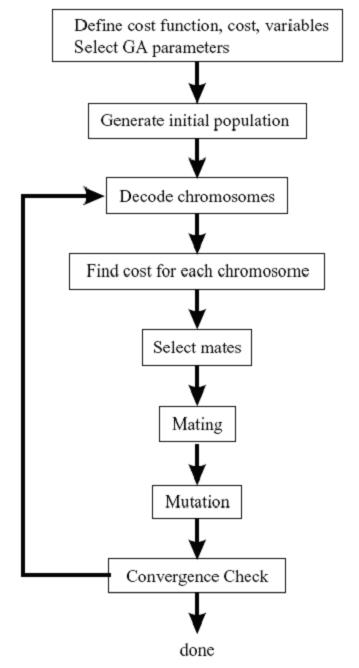
\includegraphics[height=0.5\textwidth]{fig/genetic.png}
    \end{center}
    \caption{Diagram representing phases in genetic algorithm evaluation}
    \label{fig:genetic_scheme}
\end{figure}

Genetic algorithms are widely used as a search techniques in the various fields. 
In this thesis it will be used for finding an optimal cuts in the attribute space and to 
apply attribute reduction. The success of a genetic algorithm can be quantified by estimating 
the cost, time required and the quality of final obtained solution. 

In the literature there can be found many examples of how GA is useful in solving hard 
optimizations problems, but beside unquestionable advantages there also exist downsides. 
A traditional GA without any diversity maintenance mechanism often suffers from getting 
stuck on the suboptimal peaks, because almost the entire GA population would have converged 
to a single peak, as a result of the rapid loss of population diversity \cite{bib44}, \cite{bib45}. 

There is a great deal of work showing how to set the optimal parameters in an evolutionary 
algorithm to obtain required speedup and solution accuracy, but this is not the main issue 
in this thesis. For more exact information see \cite{bib42}, \cite{bib43}.

When designing genetic algorithm one of the most important things to ensure proper crossover 
and mutation operations. More precise information about these operators will be
presented in section \ref{cha:Algorithm_construction}.

\subsection{Hybrid classifiers} 
\label{cha:Hybrid_classifiers}
In the recent years, there is an increasing interest in methods of combining
multiple learning systems into hybrid one \cite{bib5}, \cite{bib6}. The main advantage of such approach
is its ability to find different explanation for the dataset for each
classifier. If classifiers make errors on different parts of the feature space
it is possible that the ensemble of classifiers will complement each other and
the final classification will be better. 

Generally, there are two types of hybrid classifiers (example presented in fig.
\ref{fig:hybrid}:
\begin{enumerate}
    \item multiexpert systems- classifiers work in parallel, each of them is
        trained and tested on the same data and independent decisions are
        combined to compute the final result. The most common example is a
        majority voting.
    \item multistage systems- classifiers are connected in a sequence where the
        next classifier is trained and used for classification only if the
        previous classifier rejected the pattern. 
\end{enumerate}
It is hard to determine which approach is the best. Each system has its pros
and cons and the choice depends of the type of dataset and available
classifiers. In this thesis the second approach is implemented where the first
segment is built by rough sets classifier and the second one is constructed by
fuzzy logic.
\begin{figure}[H] 
    \begin{center}
        \includegraphics[width=\textwidth]{fig/hybrid.png}
    \end{center}
    \caption{Example of two approaches for constructing hybrid classifiers}
    \label{fig:hybrid}
\end{figure}



\section{Introduction into Parallel Genetic Algorithms}
\label{cha:teoria}
\subsection{Basic notation used in $\mathcal{GA}$}
\label{cha:BasicNotation}
$\mathcal{GA}$ (Genetic Algorithm) is a search algorithm inspired by genetics and
natural selection. At first it is worth introducing few basic notions connected
with this topic \cite{bib10}:
\begin{itemize}
	\item Reproduction is the process by which the genetic material in two or
		more parent individual is combined to obtain one or more offspring.
	\item Mutation is applied to one individual in order to produce a new
		version of it where some of the original genetic material has been
		randomly changed
	\item Fitness evaluation is the step in which the quality of individual is
		assessed.
	\item Selection is an operation used to decide which individuals use for
		reproduction
	\item Crossover is the basic genetic operator; it randomly chooses at least two
		individuals and with a given probability exchanges their genomes to
		create new individuals. 
	\item Offspring population- population which was created by the work of
		genetic operators.
	\item Gene- rudimentary unit building the chromosome. It encodes information
		about individual
	\item Chromosome- unit which builds the genotype of the individual, contains
		information used to identify phenotype and it can encode additional
		parameters which are not used in fitness evaluation. 
	\item Genotype- information about the individual which directly defines its
		positions in the solution space 
	\item Environment- entire solution space defined according to the problem to solve. 
\end{itemize}

\subsection{Multiprocessor system taxonomy}
\label{cha:MultiprocessorTaxonomy}
There are many ways to classify parallel computers \cite{bib20}. One of the most widely used
classification, known since 1966, is called Flynn's Taxonomy \cite{bib15}. It distinguishes
multi-processor architecture by taking into account two independent domains.
They are instruction and data domains with two possible states: Single or Multiple. This topic is
very important in case of parallel genetic realisation, but this area fall
outside the scope of this thesis. Summary presented
below is only placed here to enlighten the problem.
We can distinguish four basic combinations:
\begin{enumerate}
	\item Single Instruction, Single Data $\mathcal{SISD}$
		\begin{enumerate}
			\item A serial (non-parallel) computer 
			\item Single instruction: only one instruction stream is being acted on the CPU during any one clock cycle 
			\item Single data: only one data stream is being used as input during any one clock cycle 
			\item Deterministic execution 
			\item This is the oldest and even today, the most common type of computer 
		\end{enumerate}
	\item Single Instruction, Multiple Data $\mathcal{SIMD}$
		\begin{enumerate}
			\item A type of parallel computer 
			\item Single instruction: All processing units execute the same instruction at any given 
				clock cycle 
			\item Multiple data: Each processing unit can operate on a different data element 
			\item Best suited for specialized problems characterized by a high degree of regularity, 
				  such as graphics/image processing. 
			\item Synchronous (lockstep) and deterministic execution 
			\item Two variants: Processor Arrays and Vector Pipelines 
		\end{enumerate}
	\item Multiple Instruction, Single Data $\mathcal{MISD}$
		\begin{enumerate}
			\item A single data stream is fed into multiple processing units. 
			\item Each processing unit operates on the data independently via independent instruction streams.
		\end{enumerate}
	\item Multiple Instruction, Multiple Data $\mathcal{MIMD}$
		\begin{enumerate}
			\item Currently, the most common type of parallel computer. Most modern computers fall into this category. 
			\item Multiple Instruction: every processor may be executing a different instruction stream 
			\item Multiple Data: every processor may be working with a different data stream 
			\item Execution can be synchronous or asynchronous, deterministic or non-deterministic 
		\end{enumerate}
\end{enumerate}

\subsection{Overview of $\mathcal{PGA}$ taxonomy }
\label{cha:PgaTaxonomy}

\subsubsection{Sequential versus parallel $\mathcal{GA}$ implementations}
\label{cha:GaDifference}
When using the term parallel genetic algorithm it is important to distinguish between parallel models,
their (parallel or sequential) implementation, and the computer hardware
parallelization \cite{bib20}. A traditional sequential $\mathcal{GA}$ model has a single population and no restrictions
upon which strings recombine with which. In a parallel $\mathcal{GA}$ model there are either multiple
populations (an island model) or a~partitioning of a single population (often called a fine-grained model). 
Both parallel and sequential $\mathcal{GA}$ models can have parallel or sequential implementations.
A~sequential implementation of the global model is the traditional approach discussed 
in the literature. One process, running on a uniprocessor, performs all the calculations. 
In a~parallel implementation of the global model the steps of the $\mathcal{GA}$ (some or all of selection, crossover,
mutation, and fitness calculation) are executed simultaneously by multiple
processes running on a~parallel computer or workstation network.
In a~sequential implementation of a parallel $\mathcal{GA}$ model, multiple processes, each
responsible for a~subpopulation or partition of the full population, time share the processor 
of the uniprocessor they are running on. In a~parallel implementation of a~parallel $\mathcal{GA}$ model, 
there are multiple processes which each runs on a unique processor of a~parallel computer or workstation network.


\subsubsection{$\mathcal{PGA}$ types}
\label{cha:PgaTypes}
The basic idea behind parallel algorithm realisation is to divide solution space
into smaller parts and assign it to independent CPU units(in this thesis called
slaves). In the literature this method is called ``divide and conquer'' and can be implemented in many ways. In
this paragraph it is presented short overview of available $\mathcal{PGA}$
realisations. The way in which $\mathcal{GA}$ can be parallelized depends on few
elements:
\begin{enumerate}
	\item How individuals fitness is evaluated and mutation is applied 
	\item If the algorithm uses single or multiple population. In case of
		multiple population there is an additional question of how often migration
		is taking place
	\item How selection is applied, globally or locally
\end{enumerate}
In the literature there are many method of parallelizing $\mathcal{GA}$, but
generally the classification is as follows, according to \cite{bib10}:
\begin{enumerate}
	\item Master-Slave parallelization- this method is also known as global
		parallelization or distributed fitness evaluation. The algorithm uses a
		single population and evaluation of the individual and genetics
		operators are performed in parallel. The master stores the population
		and slaves evaluate the individuals fitness, apply mutation and make crossover
		procedure. Two versions of this algorithm can be listed:
		\begin{enumerate}
			\item Asynchronous- in this version master does not stop to wait for
				any slaves to receive the fitness evaluation.
			\item Synchronous- master stops and waits to receive the  fitness
				values for all the population before proceedings with the next
				generation. A synchronous master-slave has the same properties
				as a simple $\mathcal{GA}$
		\end{enumerate}
	\item Static Subpopulation with migration- This parallelization method requires 
		the division of a population into some number of demes. Demes
		 are separated from one another (geographic isolation), and individuals compete only
		 within a deme. An additional operator
		 called migration is introduced: from time to time, some individuals are moved 
		 from one deme to another. If individuals can migrate to any other deme, 
		 the model is called
		 an island model. If individuals can migrate only to neighbour demes, it
		 is a stepping stone model. In this class there are two main subclasses:
		 \begin{enumerate}
			 \item Coarse grained algorithm- it is a general term for a
				 subpopulation model wit a relatively small number of demes with
				 many individuals. 
			 \item Fine grained algorithm- it is the opposite of the previous
				 one. It requires a large number of processors because the
				 population is divided into a large number of small demes. 
		 \end{enumerate}
		
	\item Static overlapping subpopulations (without migration)- this type of
		algorithm resembles the previous one, but significant difference is in
		the process of migration. Propagation and exchange of traits is done by
		individuals which lie in overlapping areas in which some kind of
		interaction is possible between individuals from different
		subpopulations. 
	\item Massively parallel genetic algorithms- in this algorithm there is only
		one population, but there exists overlapping of demes which creates
		limited possibility of interaction between individuals. 
	\item Dynamic demes (dynamic overlapping subpopulations)- it is a new method
		which connects two known solutions- global parallelism and overlapping
		subpopulation model. In this model there is no migration because
		information is exchanged between the whole population. 
	\item Parallel steady-state genetic algorithms- this kind of $\mathcal{GA}$ uses
		continuous population-update schema. The only thing to deal with is the
		problem of critical section used for selection and replacement
	\item Parallel messy genetic algorithms- it has three phases. In the first
		two the initial population is created and is reduced in the process of
		selection. As the final step, partial solutions found earlier are mixed
		together
	\item Hybrid methods of $\mathcal{PGA}$- it uses combination of methods
		previously described 
\end{enumerate}


\subsubsection{Master-slave $\mathcal{GA}$- mathematical analysis}
\label{cha:PgamathematicTheory}
In the case of heuristic algorithms it is a~great problem with parameters
settings. Very often they are tuned randomly and that approach can result in
inefficient use of computing resources and poor quality solution. In case of
$\mathcal{GA}$ the main problem is with the size of population or if to use one or
multiple populations. If the population is too small, there might
not be an adequate supply of chromosomes, and it will be difficult to identify good
solutions, while on the other hand, if the population is too big the $\mathcal{GA}$ will waste
time on processing individuals fitness, and this may result in unacceptably
slow performance. The same problems are encountered in parallel $\mathcal{GA}$, and
therefore the results of the next section are crucial to answer how
to implement an efficient parallel $\mathcal{GA}$ \cite{bib1}, \cite{bib18},
\cite{bib19}. The main milestone question 
which arises in this dissertation is the relationship between the number of
slaves units, size of the population and the potential speedup resulting from parallelization.
This paragraph presents a lower bound on the potential speedup of parallel
$\mathcal{GA}$.

Before going to the core of the problem few assumption must be made to
successfully introduce mathematical formulas. Firstly, master
slave-$\mathcal{MSPGA}$ is taken into account and secondly it is assumed that the time used
by selection and crossover operations are relatively small comparing to the time
needed for communication between CPU, so can be ignored. Additionally, it is
considered that the size of population assigned to each processor is the same. 

In case of $\mathcal{MSPGA}$ time of algorithm execution is applied to the master
processor, which is connected with $\mathcal{S}$ slaves used to evaluate its population. The process of
evaluation starts when the master sends a fraction of the population to each
slave, using time $T_c$ to communicate with each. Next the master
evaluates a fraction of population using time $T_m$ described as:
\begin{equation}
	T_m=\frac{n\cdot T_f}{P}
	\label{master}
\end{equation}
where $T_f$ is the time to evaluate single individual, $n$ is the size of
population and $P=S+1$ is the number of processors(including the master unit). 
Additional time is required for each slave processor to finish its evaluation
process and resend results to the master. It can be denoted as:
\begin{equation}
	T_s=P\cdot T_c
	\label{slave}
\end{equation}
According to equations (\ref{master}), (\ref{slave}) the whole time needed to rework
entire population is as follows:
\begin{equation}
	T_p=T_m+T_s=P\cdot T_c+\frac{n\cdot T_f}{P}
	\label{total}
\end{equation}

\begin{figure}[!htb]
	\begin{center}
		\includegraphics{rys/speedUp}
	\end{center}
	\caption{Relationship between number of processors and time for
	$\mathcal{GA}$ evaluation}
	\label{fig:speedUp}
\end{figure}

Looking at the equation (\ref{total}) and figure \ref{fig:speedUp}, it is obvious that more slave processors
result in decrease of computation time, but on the other hand there is an
increase in time needed for communication between processor. To find the optimal
number of CPU to minimise total time $T_p$, gradient can be calculated in the
direction of $P$. 
\begin{equation}
	P^*=\sqrt{\frac{n\cdot T_f}{T_c}}
	\label{gradient}
\end{equation}

The main concern from equation (\ref{gradient}) is that any gain from parallel
implementation of $\mathcal{GA}$ may be squandered by frequent communication
between master and slaves. 
To ensure the speedup($S_p$) of parallel $\mathcal{GA}$ relative to sequential  $\mathcal{GA}$
the following condition must be fulfilled:
\begin{equation}
	S_p=\frac{T_s}{T_p}=\frac{n\cdot T_f}{\frac{n\cdot T_f}{P}+P\cdot
	T_c}=\frac{n\cdot \gamma}{\frac{n\cdot \gamma}{P}+P} > 1
	\label{zaleznosc}
\end{equation}
where $\gamma=\frac{T_f}{T_c}$, $T_s$ sequential
$\mathcal{GA}$ duration and $T_p$ parallel $\mathcal{GA}$ duration. 
Using equation (\ref{zaleznosc}) universal condition can be formulated to find how
the number of parallel processors affects the algorithm duration relative to the
sequential $\mathcal{GA}$ counterpart. 

\begin{equation}
	\gamma>\frac{P^2}{n(P-1)}
	\label{condition}
\end{equation}

Looking at the constant $\gamma=\frac{T_f}{T_c}$, it is obvious that parallel
genetic algorithms are profitable in situations when $T_f$ is much greater than
$T_c$. Taking into account that complexity of problems where  $\mathcal{GA}$ are
applied is great, so to obtain valuable solution it requires huge processor
computation capacity mainly to evaluate
individuals fitness, in the consequence $T_f$ is
much greater than $T_c$.


At the end of this paragraph it is worth looking at constant $T_c$. In
calculation it was assumed that this value was constant, but in a~real environment
it depends on the size of data to send, available operating system and hardware. To be
more precise in calculations, time spent on communication between master and
slave should be taken into account(time to send fraction of population form
master to slave $T_{send}$ and time to resend fraction of population from
slaves to master $T_{rec}$). Below, there are presented formulas estimating
$T_{send}$ and $T_{rec}$:
\begin{equation}
	T_{send}=B\cdot \frac{n\cdot l_i}{P}+L
	\label{send}
\end{equation}

\begin{equation}
	T_{rec}=B\cdot \frac{n\cdot l_f}{P}+L
	\label{rec}
\end{equation}
where $B$ is the throughput of the link, $L$- idle time waiting for
communication procedure,  $l_i$-message length from master to
slave, $l_f$-message length from slave to master.
Now the total time of the parallel $\mathcal{GA}$ evaluation is equal to:
\begin{equation}
	T_p=S\cdot T_{send}+T_{rec}+\frac{n\cdot T_f}{P}
	\label{total2}
\end{equation}

After repeating procedure in which equation (\ref{total}) was obtained, now the
optimal $P^*$ is described by such a following formula:
\begin{equation}
	P^*=\sqrt{\frac{n[T_f+B\cdot(l_f-l_i)]}{L}}
	\label{optimal}
\end{equation}
Assuming that parameter $B$ is very small in today communication
technique(FastEthernet, GigabitEthernet),
equation (\ref{optimal}) resembles the previous one, described by
(\ref{gradient}).

Another important issue to reconsider in this paragraph is the processor
utilization ratio. According to \cite{bib1}, the efficiency of a parallel
program is defined as the ratio of the parallel speed up over the number of
processors.
\begin{equation}
	E_f=\frac{T_s}{T_p\cdot P}
	\label{efficiency}
\end{equation}
Ideally the efficiency should be one, but the cost of communication and idle
waiting on commands causes the efficiency to decrease as more processors
are used. Now arises the question what is the critical number of slaves units to
maintain a predetermined efficiency. Equation (\ref{determinedEfficiency})
describes critical number of processors~$P_c$:
\begin{equation}
	P_c=\sqrt{\frac{1-\widehat{E_f}}{\widehat{E_f}}}\cdot\sqrt{\frac{n\cdot
	T_f}{T_c}}
	\label{determinedEfficiency}
\end{equation}
where $\widehat{E_f}$ is the predetermined efficiency. 

When $\widehat{E_f}=0.5$, which means that half of the time is devoted for computation 
and the second one processor is idle because of communication process, number of processors
described by equation (\ref{determinedEfficiency}) is the same as in case of
equation (\ref{gradient}). As the final conclusion, looking at
the~$\widehat{E_f}=0.5$~it should be possible to develop better master-slave
implementations of $\mathcal{GA}$ algorithm than the lower bound described in
this section especially in the case of communication cost which were supposed to
take half of algorithm duration time.

\subsubsection{Multi-Deme $\mathcal{GA}$-mathematical analysis}
\label{cha:CoarsedGa}
In the previous chapter there were conclusions made about master-slave parallel
$\mathcal{GA}$, in this part so called ``island model'' is taken into account.
According to \cite{bib21} it is difficult to implement this kind of algorithm
and the main issues to reconsider are as follows:
\begin{enumerate}
	\item the size and the number of demes
	\item the topology that interconnects the demes
	\item the migration rate that controls how many individuals to migrate
\end{enumerate}
% zrobic odniesienie do 24
% opisac speedup w porownaniu z sequential GA
% moze nawet pokusic sie o wykres tego.
In the literature there are two bounding cases presented \cite{bib24}. The first
one is a set of simple $\mathcal{GA}$ running in parallel with no interactions between them,
while the second one presumes that each deme exchanges individuals with all the
others, so the migration rate is set to a maximum value. 

The first bounding case of parallel $\mathcal{GA}$ considers that the demes
evolve in complete isolation, with no communication so the migration rate is
zero. There arises the question how many isolated demes is needed to get the
required solution quality. According to \cite{bib21} the quality of solution is
measured as the number of partitions $X$ that converge correctly to the global
solution, under the assumption that partitions are independent from each other.
This situation can be characterized by a binomial distribution with parameters $m$(size of the
genotype) and $P_{bb}$(probability of making the right decision between genome 
which fits and genome which does not fit to the global solution). The quality of
solution from $r$ subpopulation can be described as follows:
\begin{equation}
	X_1 < X_2 \ldots < X_r
	\label{statystyka}
\end{equation}
Now, it is expected that the best solution found in $r$ demes $X_r$ would be
equal to the desired quality described as $\hat{Q}$. The binomial distribution
of the quality can be approximated with Gaussian distribution and the number of
the correct partitions in each deme is normalized as:
\begin{equation}
	z_i=\frac{X_i-m\cdot P_{bb}}{\sqrt{m\cdot P_{bb}\cdot(1-P_{bb})}}
	\label{zi}
\end{equation}
Having the equation (\ref{zi}), the expected quality of the best deme can be
described as follows
\begin{equation}
	E(z_r)=\mu_{r:r}
	\label{Ez}
\end{equation}
where $\mu_{r:r}$ is the mean of the highest-order statistic of a standard normal
distribution. The expected value of $X_r$ is, according to \cite{bib21}
\begin{equation}
	\hat{Q}=E(X_r)=m\cdot P_{bb}+\mu_{r:r}\sqrt{m\cdot P_{bb}\cdot(1-P_{bb})}
	\label{Q}
\end{equation}
Setting $P_{bb}=0.5$ in (\ref{Q}) the bounding case can be calculated as
follows:
\begin{equation}
	\hat{Q}=E(X_r)=m\cdot P_{bb}+\frac{\mu_{r:r}}{2}\sqrt{m}	
	\label{p0.5}
\end{equation}
Having the equation (\ref{p0.5}), it is high time to calculate the required probability
of convergence to the global optimum for each subpopulation and after that one of
the most important thing which is the size of population for each slave. 
\begin{equation}
	\hat{P}=\frac{\hat{Q}}{m}-\frac{\mu_{r:r}}{2\cdot\sqrt{m}}
	\label{P}
\end{equation}
To find the deme size, the Gambler's ruin problem must be introduced to describe
$\hat{P}=P_{bb}$(more information about Gambler's ruin problem can be found in
\cite{bib26}). Equation (\ref{P}) must be solved for $n_d$, where
$P_{bb}=1-(\frac{q}{p})^{\frac{n_d}{2^k}}$
\begin{equation}
n_d=\frac{2^k\cdot\ln(1-\hat{P})}{\ln(\frac{q}{p})}
	\label{nd}
\end{equation}

The best way to compare parallel and sequential $\mathcal{GA}$ is to express
serial and parallel times required to find a solution as the parallel speedup
$S_p$. 
\begin{equation}
	S_p=\frac{g\cdot n\cdot T_f}{g\cdot n_d \cdot T_f}=\frac{n}{n_d}
	\label{speedUpDeme1}
\end{equation}
where $g$ stands for the number of generations.

The first part of this paragraph described the lower bound for parallel
$\mathcal{GA}$ because the migration rate is zero and there are no connections
between the demes. Now, the analysis consider that migration factor is equal to~1 
and subpopulations are connected with each other. Again these problems can be
divided into few subdomains with bounding cases, for example how often the
migration process is taking place:
\begin{itemize}
	\item in every generation
	\item after the convergence of subpopulation
\end{itemize}
Here, the analysis consider that migration occurs where all the individuals in
each deme are identical(converged). When that situation is taking place, each deme divides
its population into $r$ sets and exchange the individuals of the $i$~set with
the $i$~deme. According to \cite{bib21}, the probability that a partition
converges to the correct value in sequential $\mathcal{GA}$ is predicted by the
equation:
\begin{equation}
	P_{bb}=1-(\frac{q}{p})^{x_0}
	\label{pbb}
\end{equation}
where $x_0$ is the expected number of genomes in the partition. When deme
converges the first time, a partition either has $n_d$ copies of the correct value
with probability $P_{bb}$, or it has $n_d$ copies of the wrong value with probability
$1-P_{bb}$. After convergence each deme receives $n_d/r$ migrants from every other
deme, some of those migrants contain the wrong value, but some have the
correct one. Therefore, after migration each partition has on average
$n_d\cdot P_{bb}$ copies of the correct value, which means that the second epoch starts from a
better starting point than the first. To calculate the probability that the deme
converges correctly the second time the Gambler's ruin model\cite{bib26} may be used
again with one exception, because $x_0$ introduced in (\ref{pbb}) must be
replaced with the new starting point.
\begin{equation}
	P_{bb2}=1-(\frac{q}{p})^{n_d\cdot P_{bb}}
	\label{pbb2}
\end{equation}

The required deme size for the fully connected topology will be calculated
next using a procedure similar to the one used for the isolated case. The first
step is to calculate the relaxation of the quality required in each deme so that
the best of the demes reaches the desired solution. This was already done in
the previous section, and the result is denoted by $\hat{P}$. Now it is time to
solve  $\hat{P} = P_{bb2}$ for the deme size $n_d$. Equation (\ref{pbb2}) can be 
approximated as: $P_{bb2} = 1 - (1 - c)^{n_d\cdot P_{bb}}$
where $c=1-q/p$, and in this form $P_{bb2}$ is as follows
\begin{equation}
	P_{bb2}\approx 1-\exp(-c\cdot n_d \cdot P_{bb})
	\label{approx}
\end{equation}
Similarly, $P_{bb}$ can be rewritten exactly as $P_{bb}=1-(1-c)^{n/2^k}$ and approximated
by $P_{bb} = 1 - \exp(-cn/2^k)$ . Using the first two terms of the Maclaurin series for
$\exp(-x)=1 - x$, $P_{bb}$ can be roughly as $P_{bb}\approx
\frac{cn}{2^k}$. Substituting this form of $P_{bb}$ into equation (\ref{approx}) it results in:
\begin{equation}
	P_{bb2}\approx 1-\exp(\frac{-c^2n^2_d}{2^k})
	\label{approx2}
\end{equation}
With this form of $P_{bb2}$ it is possible now to solve $\hat{P} = P_{bb2}$ to
find $n_d$-a~deme size for a~fully connected topology:
\begin{equation}
	n_d=\frac{\sqrt{-2^k\cdot\ln(1-\hat{P})}}{1-\frac{1}{p}}
	\label{nd2}
\end{equation}

Now it is time to compare obtained results from equation (\ref{nd}) and
(\ref{nd2}). In the fully connected demes, the deme size depends on 
the square root of $2^k\ln(1-\hat{P})$ as opposed to the
case for isolated demes where it is directly proportional to this
term. This shows that a parallel  $\mathcal{GA}$ with migration needs smaller demes,
which in turn represents a substantial reduction of the time the $\mathcal{GA}$ uses in
computations. But on the other hand there is the issue of communication to
reconsider, which will be taken care of in the next paragraph. 

The time that each deme uses to communicate with its $r-1$ neighbors is
$(r-1)\cdot T_c$; and the time used in computations is $g\cdot n_d\cdot T_f$ ,
so the execution time of the parallel program is as follows:
\begin{equation}
	T_p=(r-1)\cdot T_c+g\cdot n_d\cdot T_f
	\label{tcomP}
\end{equation}
To optimize the parallel execution time, $\frac{\partial T_p}{\partial r}$ has to be
calculated to obtain the optimal number of demes. Unfortunately, the derivative
cannot be solved analytically for $r$. According to \cite{bib21} the parallel
deme size can be characterized by a simpler expression and equation
(\ref{tcomP}) can be transformed into:
\begin{equation}
	T_p=(r-1)\cdot T_c+g\cdot A\cdot r ^B \cdot T_f
	\label{tcomP2}
\end{equation}
Now it is possible to evaluate $\frac{\partial T_p}{\partial r}=0$ to obtain the
optimal number of demes 
\begin{equation}
	r^*=(-\frac{g\cdot A\cdot B\cdot T)f}{T_c})^{\frac{1}{1-B}}
	\label{rOptimal}
\end{equation}
and the optimal deme size(as described in \cite{bib21}) is 
\begin{equation}
	n^*_d=A\cdot r^{*B}
	\label{ndOptimal}
\end{equation}
where A and B are domain-dependent constants.

\subsubsection{Other types of $\mathcal{PGA}$}
In the previous section there were presented the most common types of
$\mathcal{PGA}$, but it is worth emphasising that this is one of~many possible
divisions and criteria which can be met in the literature. In this paragraph
there will be shown two additional types but without the precise mathematical
analysis about possible speedup because cases described previously( section
\ref{cha:PgamathematicTheory},\ref{cha:CoarsedGa}) are the lower
and upper bound respectively. It is not the intention to describe them in
detail, but to show their existence. 

The first characteristic is about fine-grained parallel genetic algorithm. In
this case the base population is divided into subpopulations with small number
of representatives. In this algorithm there is relatively great number of
subpopulation which requires constant communication between them. One noticeable
advantage of this solution is a~quite fast disperse of good solution in the entire
population. 

The second one is the hybrid genetic algorithm which is the connection of
algorithms presented earlier in this section. It uses many populations in which
every subpopulation is the form of parallel genetic algorithm. To fully
understand the architecture of this solution, illustration \ref{fig:hybrid}
was presented.
\nopagebreak
\begin{figure}[!htb]
	\begin{center}
		\includegraphics{rys/hybrid}
	\end{center}
	\caption{Hybrid parallel genetic algorithm-schematic illustration}
	\label{fig:hybrid}
\end{figure}


\newpage
\section{Experimentation system}
\label{cha:ExperimentAnalysis}
\subsection{Assumptions}
This section starts the second part of this thesis. In the first it was proved
that for the certain parameters settings it is advisable to use parallel genetic
algorithm instead of sequential one. There were formulas presented showing the
optimal number of slaves for master-slave and deme configuration. The main goal
of this part is to check how other parameters(not only number of slave units)
affects efficiency of tested algorithm. Experiments were carried out to compare 
required time to run the same $\mathcal{GA}$
sequentially on a single machine against the time it takes to run on the
distributed environment, to find out what is the quality of solution in both cases and try to answer 
the question when and in what situation it is reasonably to use parallel
genetic algorithms.

For this project there were three genetic algorithms implemented, one simple
sequential program and two parallel counterparts. 
\begin{itemize}
	\item Sequential genetic algorithm, it is the basic algorithm with one
		population and standard method of selection, mutation and replacement.
	\item Parallel genetic algorithm with the ``island'' model. It was assumed
		that there is one master program which triggers the slave processes and
		collects the final results from them.
		Additional assumption is that each slave has its own population to
		evaluate and occasionally sends individuals to other units in the process
		of migration. There are two possible migration types: the first denoted
		as PGA\_f assumes that migration is to the forward neighbour, while the
		second one-PGA\_b sends its genomes in both directions. Described here
		topologies were presented in figure \ref{fig:topology}
\end{itemize}
\begin{figure}[!htpb]
	\begin{center}
		\includegraphics[width=\textwidth]{rys/topology}
	\end{center}
	\caption{Schematic topology for PGA\_f(on the left) and PGA\_b}
	\label{fig:topology}
\end{figure}
At the beginning of the project it was a problem to choose a reliable environment
to perform all tests. One possible solution was to set LAN network but because
of shortage of time and resources different approach was applied. In all researches
pvm(Parallel Virtual Machine) framework was used to virtualize slave units. One 
computer played the role of master CPU and later started other processes. This is 
maybe not the most reliable environment but to perform basic tests and simulate
communication and migration between slave units it is enough. Of course there 
are programs ready to use, for
example Matlab software, but in those cases they only simulate multideme population
on one processor where algorithm is run sequentially, so it would
not be possible to check parallel program speedup to the sequential one.
In that situation it was advisable to write special program for project's purposes.


Implemented algorithms were used to solve optimization problem which required
finding the global minimum in test functions. This approach is very often used
to check if algorithm is resistant to falling into one local minimum as a result
of small diversity in population. Genetic algorithms have stochastic nature so each
simulation was repeated 200 times and every time individuals were encoded using
the floating point representation.


\subsection{Test functions}
\label{cha:function}
In the introduction it was said that the most important thing in implementing
the parallel genetic algorithm is the ratio $\frac{T_f}{T_c}$, to ensure that time spent on
genome fitness evaluation must be much longer than time wasted on communication
between slaves units. For that reason costly effective functions will be used in this
project, chosen from \cite{bib25}. 
Objective functions to evaluate effectiveness of algorithm implementation are De Jong's 
functions(very often used in the literature to check performance of
$\mathcal{GA}$ algorithms) which will be listed below with a~priori known global
minimum(This information was used in the project to compare with results
obtained by designed program) 
\begin{enumerate}
\item De Jong's function-F1(four variables)
	\begin{equation}
		F(\underline{x})=\sum_{i=1}^n x^2_i; \textnormal{  } \bigvee_i x_i \in
		[-5.12, 5.12]
		\label{dj1}
	\end{equation}
	where $\min(F(x_1,x_2,x_3,x_4))=F(0,0,0,0)=0$
	\nopagebreak
	\begin{figure}[!htpb]
		\begin{center}
			\includegraphics{rys/F1}
		\end{center}
		\caption{Visualisation(for two variables) of De Jong's function-F1}
		\label{fig:F1}
	\end{figure}
\item De Jong's function-F2(two variables)
	\begin{equation}
		F(\underline{x})=\sum_{i=1}^{n-1}100\cdot(x_i^2-x_{i+1})^2+(x_i-1)^2;
		\textnormal{  } \bigvee_i x_i \in [-5.12,5.12]
		\label{dj2}
	\end{equation}
	where $\min(F(x_1, x_2))=F(1,1)=0$
	\pagebreak
	\begin{figure}[!htpb]
		\begin{center}
			\includegraphics{rys/F2}
		\end{center}
		\caption{Visualisation(for two variables) of De Jong's function-F2}
		\label{fig:F2}
	\end{figure}
\item De Jong's function-F3(four variables)
	\begin{equation}
		F(\underline{x})=\sum_{i=1}^n\lfloor x_i \rfloor ; \textnormal{  }
		\bigvee_i x_i \in [-5.12,5.12]
		\label{dj3}
	\end{equation}
	where $\min(F(x_1,x_2,x_3,x_4))=F(-5.12, -5.12, -5.12, -5.12)=-24$
	\nopagebreak
	\begin{figure}[!h]
		\begin{center}
			\includegraphics{rys/F3}
		\end{center}
		\caption{Visualisation(for two variables) of De Jong function-F3}
		\label{fig:F3}
	\end{figure}
\item De Jong's function-F4(four variables)
	\begin{equation}
		F(\underline{x})=\sum_{i=i}^n i\cdot x_i^4+\textnormal{gauss(0,1)}; \textnormal{  }
		\bigvee_i x_i \in [-1.028, 1.028]
		\label{dj4}
	\end{equation}
	where $\min(F(x_1, x_2, x_3, x_4))=F(0, 0, 0, 0)=0$
	\nopagebreak
	\begin{figure}[!htpb]
		\begin{center}
			\includegraphics{rys/F4}
		\end{center}
		\caption{Visualisation(for two variables) of De Jong function-F4}
		\label{fig:F4}
	\end{figure}

\item De Jong's function-F5(two variables)
	\begin{equation}
		F(\underline{x})=\frac{1}{K}+\sum_{j=1}^{26}\frac{1}{j+\sum_{i=1}^2(x_i-a_{ij})^6}; \textnormal{  }
		\bigvee_i x_i \in [-5.12,5.12]
		\label{dj5}
	\end{equation}
	\begin{small}	
	\[a_{ij}=\left ( \begin{array}{cccccccccc}
  -32& -16& 0& 16& 32& -32& \ldots & 0& 16& 32\\
  -32& -32& -32& -32& -32& -16& \ldots& 32& 32& 32
		\end{array} \right )\]
	\end{small}
	where $\min(F(x_1, x_2))=F(-32,-32)=1$
	\pagebreak
	\begin{figure}[!htpb]
		\begin{center}
			\includegraphics{rys/F5}
		\end{center}
		\caption{Visualisation(for two variables) of De Jong's function-F5}
		\label{fig:F4}
	\end{figure}

\item Rastring's function-F6(seven variables)
	\begin{equation}
		F(\underline{x})=\sum_{i=1}^nx_i^2+ 10\cdot
		(n-\sum_{i=1}^{n}\cos(2\cdot\pi\cdot x_i)) \textnormal{
		} \bigvee_i x_i \in [-20, 20]
		\label{r5}
	\end{equation}
	where $\min(F(x_1, x_2, \ldots, x_7))=F(0,0,\ldots, 0)=0$
	\nopagebreak
	\begin{figure}[!htpb]
		\begin{center}
			\includegraphics{rys/F6}
		\end{center}
		\caption{Visualisation(for two variables) of Rastrings's function-F6}
		\label{fig:F5}
	\end{figure}
\end{enumerate}
\subsection{Efficiency indicators}
\label{cha:indicators}
To evaluate effectiveness of algorithm it has to be consistent approach used in
all experiments and additionally the a~priori global minimum value has to be taken
into account. Below, there will be listed methods of algorithm fitness scoring
\begin{itemize}
	\item An absolute error which is the distance between the solution found by
		algorithm and known a~priori global minimum. There are distinguished
		three variants of this indicator
		\begin{itemize}
			\item The best value from $n$ probes 
				\begin{equation}
					B=MIN\left | f^{*}(\underline{x})-f(\underline{x}) \right |
					\label{min1}
				\end{equation}
			\item The worst value from $n$ probes 
				\begin{equation}
					W=MAX\left | f^{*}(\underline{x})-f(\underline{x}) \right |
					\label{min3}
				\end{equation}
			\item The average value from $n$ probes
				\begin{equation}
					A=\frac{1}{n}\sum_{n=1}^n\left | f^{*}(\underline{x})-f(\underline{x}) \right |
					\label{min2}
				\end{equation}
		\end{itemize}
		where $f^{*}(\underline{x})$ is the value found by algorithm and
		$f(\underline{x})$ is a~priori global minimum.
	\item Error variance from $n$ simulations 
		\begin{equation}
			\sigma^2=\frac{1}{n-1}\sum_{i=1}^n\left[A-B\right]^2
			\label{min4}
		\end{equation}
	\item Average time from $n$ simulation, where $T_i$ is $i-th$ simulation
		time
		\begin{equation}
			T=\frac{1}{n}\sum_{i=1}^nT_i
			\label{min4}
		\end{equation}
\end{itemize}
\subsection{Program description}
%-----------------------------------------------------------------------------------------
To perform all simulations in this project a program was written in
$\mathcal{C++}$(more information can be found in \ref{Appendix}). It allows running simple sequential and parallel genetic
algorithm. Libraries used in it are as follows:
\begin{itemize}
	\item $\mathcal{GALIB}$- library released by the Massachusetts Institute
		of Technology which is very useful in implementing $\mathcal{GA}$. In
		this library all standard operations such as replacement, crossover,
		mutation, encoding are implemented and easy to customize.
		$\mathcal{C++}$ is an objected programming language in which inheritance
		plays very important role. In program for this project basic
		functionality was taken from $\mathcal{GALIB}$ and customized so that to
		use it for simulations.
	\item pvm framework- library used to manage communication between slaves \cite{bib3}, \cite{bib13}.
		In $\mathcal{PGA}$ there was a problem of how to send individuals between
		slaves units and how to pack message buffer. In pvm communication is
		done very simply. When creating slaves by the master each of them
		receives $id$ by which is later recognized in the system. So sending 
		a~message requires giving an $id$ and a handle to the message buffer. 
	\item lpthread- library used for slave synchronization and communication.
		Mutex and mechanism called waiting on condition was implemented to
		ensure that each slave takes part in the migration process. Each slave has
		its own thread used for reading messages and after receiving
		individuals from migration it signalizes slave's process to stop and
		replace genomes. 
\end{itemize}
Program was tested on Linux system and to start it command line is required.  To
compile the project g++ compiler was used and all rules needed in compilation
and linking process were placed in \textsc{Makefile}. It is very useful solution
because instead of writing many command only one is sufficient. To be able to
run program one has to install pvm server which is responsible for starting
master program and spawning slaves. Because implemented $\mathcal{GA}$ algorithm
has many setting parameter, they were written to the file so that easily
change their value in testing procedure. Output results(efficiency indicators) were written to
\textsc{csv}. The
general project structure is presented in Fig. \ref{fig:setting}. 
\pagebreak
\begin{figure}[!htpb]
	\begin{center}
		\includegraphics{rys/box}
	\end{center}
	\caption{Schematic project structure}
	\label{fig:setting}
\end{figure}
%-----------------------------------------------------------------------------------------


\section{Investigations}
\label{cha:investigation}
\subsection{Design of experiments}
This section presents results collected from conducted simulations. In
table \ref{configuration} there are presented configuration parameters for each kind
of genetic algorithm, while the basic notation used in this paper is as follows:
\begin{itemize}
	\item SGA - simple sequential genetic algorithm
	\item PGA\_f- parallel genetic algorithm with forward migration process
	\item PGA\_b- parallel genetic algorithm where genomes are passed to
			both neighbours
	\item $\mathcal{N}$- number of slaves 
	\item fp- floating point representation
	\item F- function type 
	\item G- number of generations each algorithm was run
	\item $\mathcal{N}$- number of slaves units
	\item $\mathcal{M}$- number of genomes sent in the migration process
	\item $\mathcal{I}$- interval of migration
\end{itemize}
\pagebreak
\begin{table}[!htpb]
	\label{configuration}
	%\rowcolors{3}{tableShade}{white}
	\caption{Algorithms configuration parameters}
	\centering
	\begin{tabular}{l||c|c|c}
        \textsc{Parameter} & \multicolumn{3}{c}{Type of algorithm} \\ \hline 
		 & \textbf{SGA} & \textbf{PGA\_f} & \textbf{PGA\_b} \\ \hline
		\textsc{Generations} 	&400	&400    &400    \\ \hline
		\textsc{N} 	&-	&5    &5    \\ \hline
		\textsc{Population} 	&300	&300/$\mathcal{N}$   &  300/$\mathcal{N}$  \\ \hline
		\textsc{Replacement}    &0.25   &0.25& 0.25 \\ \hline
		\textsc{Mutation}       &0.2    &0.2 &0.2   \\ \hline
		\textsc{Crossover}      &0.7    &0.7 &0.7   \\ \hline 
		\textsc{Convergence}    &0.995  &0.995& 0.995 \\ \hline
		\textsc{Migration step- $\mathcal{I}$}      &-& 20 &20 \\ \hline
		\textsc{nMigration- $\mathcal{M}$}     &-& 10 &10 \\ \hline
		\textsc{Direction}      &-& Forward & Both \\ \hline
		\textsc{Representation} &fp&fp&fp \\ \hline
		\textsc{Repetition} &200&200&200 \\ \hline
	\end{tabular}\newline
\end{table}
Before presenting the final results, few words of comments should be made about
parameters from table \ref{configuration} and why those values were chosen in
simulations. In the literature there are many examples of parallel genetic
algorithm implementations \cite{bib22}, \cite{bib27}. In those articles applications
are fully described with detailed description of input parameters. This was the
main source of information how to set up parameters for simulations in this
project. This project is the first work in this area and because $\mathcal{GA}$ algorithm 
has many parameters settings which the influence on the algorithm result is is
non-linear, it was advisable to use tested configuration and well known in the
literature. Few additional constraints had to be taken into account. According
to \cite{bib19}, population has to be big enough to ensure diversity and
number of generation has to be chosen at reasonably rate to try to search the
greatest part of the solution space. In all experiments size of the population
was equal to $300/\mathcal{N}$, so even for great $\mathcal{N}$ algorithm
preserved individuals diversity.  
\subsection{Algorithm duration- comparison of $\mathcal{SGA}$ with
$\mathcal{PGA}$}
In this experiment three algorithms were run with the same input data and
each algorithm had configuration corresponding to \ref{configuration}. The main
purpose of this experiment was to check two indicators: time of
algorithm evaluation and accuracy of solution obtained from $\mathcal{SGA}$ and
from both types of $\mathcal{PGA}$. Results are collected in tables \ref{sga},
\ref{pga1conv}, \ref{pga2conv}. Each algorithm has stopped after gaining
convergence at $0.995\%$. 
\begin{table}[!htpb]
	\label{sga}
	%\rowcolors{3}{tableShade}{white}
	\caption{Results of $\mathcal{SGA}$ in case of algorithm duration}
	\centering
	\begin{tabular}{l||r|r|r|r|r|r|}
        \textsc{F} & \multicolumn{6}{c|}{SGA} \\ \hline
		          &T[ms]&G& B&W&A&$\sigma^2$ \\ \hline
		\textsc{F1}&32420&237&0.00160298&0.0528165&0.0121706&0.000132399\\ \hline
		\textsc{F2}&20365&148&4.96253e-06&0.00913949&0.00162763&4.45288e-06\\ \hline
		\textsc{F3}&8470&173&0&1&0.06&0.057551\\ \hline
		\textsc{F4}&14192&103&0.0759622&6.30168&1.92343&2.12657\\ \hline
		\textsc{F5}&71115&118&3.8147e-06&4.41074e-06&3.86715e-06&1.11135e-14\\ \hline
		\textsc{F6}&39785&266&5.29394&24.0324&15.4658&14.1652\\ \hline
	\end{tabular}\newline
\end{table}
\pagebreak
\begin{table}[!htpb]
	\label{pga1conv}
	%\rowcolors{3}{tableShade}{white}
	\caption{Results of $\mathcal{PGA}$ with forward migration in case of
	algorithm duration}
	\centering
	\begin{tabular}{l||r|r|r|r|r|r|}
        \textsc{F} & \multicolumn{6}{c|}{PGA\_f} \\ \hline
		          &T[ms]&G& B&W&A&$\sigma^2$ \\ \hline
		\textsc{F1}&12392&209&0.000545337&0.0180944&0.00416617&1.06863e-05\\ \hline
		\textsc{F2}&8703&165&1.27917e-06&0.0196572&0.00180196&1.86041e-05\\ \hline
		\textsc{F3}&7959&171&0&1&0.02&0.02\\ \hline
		\textsc{F4}&7469&114&0.0217737&6.14396&1.57031&2.0549\\ \hline
		\textsc{F5}&46832&134&3.8147e-06&0.204763&0.00409903&0.000838523\\ \hline
		\textsc{F6}&15710&230&4.35369&27.7749&16.2711&16.6755\\ \hline
	\end{tabular}\newline
\end{table}
\nopagebreak
\begin{table}[!htpb]
	\label{pga2conv}
	%\rowcolors{3}{tableShade}{white}
	\caption{Results of $\mathcal{PGA}$ with both neighbour migration in case of
	algorithm duration}
	\centering
	\begin{tabular}{l||r|r|r|r|r|r|}
        \textsc{F} & \multicolumn{6}{c|}{PGA\_b} \\ \hline
		          &T[ms]&G& B&W&A&$\sigma^2$ \\ \hline
			\textsc{F1}&12605&217&0.000170366&0.0116758&0.00184919&3.20086e-06\\ \hline
			\textsc{F2}&8237&156&7.60546e-07&0.0801857&0.00566568&0.000261041\\ \hline
			\textsc{F3}&8288&166&0&0&0&0\\ \hline
			\textsc{F4}&7321&111&0.0310541&6.14396&1.62028&2.02956\\ \hline
			\textsc{F5}&44475&129&3.8147e-06&0.204314&0.00409005&0.000834852\\ \hline
			\textsc{F6}&19512&273&7.50491&22.7055&13.9941&13.3396\\ \hline
	\end{tabular}
\end{table}
Looking at the result collected in tables, it can be seen that
for every function type parallel genetic algorithm finished much faster than
sequential genetic counterpart. In case of parallel genetic algorithm each slaves
has its own population with the size equal to $300/\mathcal{N}=60$ while sequential
genetic algorithm has the population of $300$ genomes so for $\mathcal{SGA}$ it takes longer to search
entire solution space. In case of $\mathcal{PGA}$ there is always a danger of
having small diversity in chromosomes where size of population is too small, but
in this case it was not a problem because $60$ individuals is relatively
sufficient number.

For $\mathcal{SGA}$ algorithm each operation (selection, migration, crossover)
is made sequentially on the entire population while for $\mathcal{PGA}$ it is
easier to obtain convergence in shorter time.

To conclude this experiment, there are collected summary results as bar
plots(figure \ref{fig:bar}). For each indicator(fully described in section
\ref{cha:indicators}) obtained results from three algorithms(
$\mathcal{SGA}$, $\mathcal{PGA}_f$,$\mathcal{PGA}_b$)were compared
and algorithm with the best result was awarded with $1$ while others with zero.
\nopagebreak
\begin{figure}[!htpb]
	\begin{center}
		\includegraphics[width=\textwidth]{rys/summary}
	\end{center}
	\caption{Final summary between $\mathcal{SGA}$ and $\mathcal{PGA}$(the
	higher the rate, the better algorithm performance) }
	\label{fig:bar}
	\newline
	\begin{itemize}
		\item 1- $\mathcal{SGA}$
		\item 2- $\mathcal{PGA}$ with forward migration
		\item 3- $\mathcal{PGA}$ with both direction of migration
	\end{itemize}
\end{figure}
Analyzing summary results from \ref{fig:bar}, it can be seen that for every
type of efficiency indicator $\mathcal{PGA}$ was better than $\mathcal{SGA}$. It is
especially very important for algorithm duration time(for every objective
function $\mathcal{PGA}$ has worked shorter than $\mathcal{SGA}$), $B$
value(always $\mathcal{PGA}$ better) and variance. Of
course it is not always true that parallel genetic algorithm has better
performance than the sequential one, its efficiency strongly depends on configurations
parameters. This is very important condition which must be remembered. How wrong
parameters setting can spoil the result, one can look at other experiments, for example in section
\ref{cha:cpu}; it can be seen that the unsuitable number of slaves($\mathcal{N}=30$) results in weak
performance of algorithm in case of algorithm duration and solution accuracy(even worse than $\mathcal{SGA}$).

In this section implemented algorithms have been tested with six test functions to
show general relationship between $\mathcal{SGA}$ and $\mathcal{PGA}$. In the
next sections only one function will be taken into account in simulations. It
will be Rastring's function(F6) because of its complexity(it has seven variables) and 
difficulty in finding good solution(it has many local minimum, but only one global
minimum).  


\subsection{Impact of slaves units number on $\mathcal{PGA}$ performance}
\label{cha:cpu}
This experiment checks how the number of slave units affects algorithm
efficiency in case of its duration and solution accuracy. There were two $\mathcal{PGA}$
algorithm types compared, one with forward and the second with both direction of
migration. Every time size of the
population was equal to 300/$\mathcal{N}$ where $\mathcal{N} \in <2, 3, 5, 7, 10,
30>$. Figure \ref{fig:cpu} and tables \ref{pga1cpu}, \ref{pga2cpu} present
collected results. Figure \ref{fig:cpu} has two plots, the first is the number of slaves in the reference of algorithm
duration and the second indicates the best absolute error value. 
\nopagebreak
\begin{table}[!htpb]
	\label{pga1cpu}
	%\rowcolors{3}{tableShade}{white}
	\caption{Results of $\mathcal{PGA}$ with forward migration with the changing
	size of population}
	\centering
	\begin{tabular}{l||r|r|r|r|r|r|}
        $\mathcal{N}$ & \multicolumn{6}{c|}{PGA\_f} \\ \hline
		          &T[ms]&G& B&W&A&$\sigma^2$ \\ \hline
		2&26603&400&4.53&17.35&10.75&6.64\\ \hline
		3&25837&400&6.67&16.79&10.89&5.99\\ \hline
		5&22734&400&4.62&18.90&10.44&10.75\\ \hline
		7&24346&400&4.01&17.81&11.40&7.08\\ \hline
		15&28842&400&3.27&18.88&11.20&11.83\\ \hline
		30&102417&400&11.71&41.82&22.55&30.74\\ \hline
	\end{tabular}
\end{table}
%\nopagebreak
\begin{table}[!htpb]
	\label{pga2cpu}
	%\rowcolors{3}{tableShade}{white}
	\caption{Results of $\mathcal{PGA}$ with both neighbour migration with the changing
	size of population}
	\centering
	\begin{tabular}{l||r|r|r|r|r|r|}
        $\mathcal{N}$ & \multicolumn{6}{c|}{PGA\_b} \\ \hline
		          &T[ms]&G& B&W&A&$\sigma^2$ \\ \hline
	2&29109&400&5.56&15.20&10.15&6.54\\ \hline
	3&27758&400&4.58&15.97&10.09&7.45\\ \hline
	5&25096&400&4.74&16.99&9.94&6.84\\ \hline
	7&33073&400&4.21&19.21&11.57&10.96\\ \hline
	15&43300&400&5.32&17.33&11.55&8.07\\ \hline
	30&104601&400&8.46&20.36&14.69&8.56\\ \hline
	\end{tabular}
\end{table}
%\nopagebreak
\begin{figure}[!htpb]
	\begin{center}
		\includegraphics[width=\textwidth]{rys/cpu_solution}
	\end{center}
	\caption{Number of slaves in the reference of algorithm duration(on the left) and solution
	accuracy}
	\label{fig:cpu}
\end{figure}
Analyzing the results it is obvious that for the specific configuration
parameters there is optimal number of slaves in case of algorithm duration. From
the certain value of $\mathcal{N}$ the expenses of communication are much greater 
than the quality of solution obtained by algorithm. In this experiment the optimal 
number of slaves is about $5$ or $7$. In case of $\mathcal{PGA}_b$ it gets the
best results for $5$~slaves not only for time indicator, but also for $B$, $A$
and it gets the most stable solution indicated by the smallest variance. For
$\mathcal{PGA}_f$ the best results were obtained for $\mathcal{N}=7$.
One of possible reason why $\mathcal{PGA}_b$ and $\mathcal{PGA}_f$ have
different optimal $\mathcal{N}$ is the type of migration. In case of $\mathcal{PGA}_f$ 
it occurs only to forward neighbour so it obtains smaller diversity as it was for
$\mathcal{PGA}_b$.


Additional conclusion can be drawn from figure \ref{fig:cpu}. Normally, everyone
would think that having the greater number of slaves can lead to the better
solution, but it is otherwise. Greater $\mathcal{N}$ implies more communication
between slaves which has a negative effect on algorithm duration(compare plot on the left 
for $\mathcal{N}=5$ and $\mathcal{N}=30$). Another aspect connected
with $\mathcal{N}$ is the size of population. As it was said before, this
relationship is as follows $300/\mathcal{N}$, so for greater $\mathcal{N}$
algorithm starts with worse diversity of chromosomes(for $\mathcal{N}=30$
algorithm obtains much worse results than for 5 or 10). 

At the end of this paragraph it has to be mentioned that algorithm performance
scoring cannot be judged only on the basis of $\mathcal{N}$ parameter but another 
settings have to be taken into account. Time of algorithm duration and solution accuracy is not only
affected by number of slaves, but additionally by number of genomes sent in the process of
migration and its interval. This will be the issue to reconsider in the next sections.

\subsection{Impact of migration interval on $\mathcal{PGA}$ performance}
The main goal of experiments presented in this section was to check how the
interval of migration affects the time of algorithm duration and other
indicators. The basic assumption here is that in every migration process
$\mathcal{M}$ the best individuals from one 
generation is send to another and replaced with $\mathcal{M}$ the worst ones. 
There arise the question, what is the best interval of migration, if it should
be very often to spread the best
genomes in the entire population, or rather rarely. On the other hand, there is always a danger
of deteriorating individuals fitness in slaves because for one slave its best
genomes could be treated as the worst for another. 

In this research migration process was evoked every $\mathcal{I}$-th algorithm
iteration, where $\mathcal{I} \in <1, 10 , 50 , 100, 200, 0>$(0 means that
there is no migration between slaves) and the rest parameters were the same as shown in
\ref{configuration}. 
\begin{table}[!htpb]
	\label{pga1step}
	%\rowcolors{3}{tableShade}{white}
	\caption{Results of $\mathcal{PGA}$ with the changing
	step of migration with one direction}
	\centering
	\begin{tabular}{l||r|r|r|r|r|r|}
        $\mathcal{I}$ & \multicolumn{6}{c|}{PGA\_f} \\ \hline
		          &T[ms]&G& B&W&A&$\sigma^2$ \\ \hline
		1&196691&400&4.99&26.95&10.40&11.73\\ \hline
		10&26673&400&5.66&18.99&10.82&8.82\\ \hline
		50&21408&400&7.13&21.96&12.80&9.53\\ \hline
		100&20625&400&5.95&21.25&14.82&9.57\\ \hline
		200&20142&400&5.84&24.01&15.93&13.27\\ \hline
		0&19803&400&7.30&23.67&17.66&13.18\\ \hline
	\end{tabular}
\end{table}

\begin{table}[!htpb]
	\label{pga2step}
	%\rowcolors{3}{tableShade}{white}
	\caption{Results of $\mathcal{PGA}$ with the changing
	step of migration in both directions}
	\centering
	\begin{tabular}{l||r|r|r|r|r|r|}
        $\mathcal{I}$ & \multicolumn{6}{c|}{PGA\_b} \\ \hline
		          &T[ms]&G& B&W&A&$\sigma^2$ \\ \hline
	1&346678&400&4.11&17.79&9.99&7.82\\ \hline
	10&70948&400&4.48&15.56&9.67&6.04\\ \hline
	50&40758&400&6.35&14.90&10.05&4.26\\ \hline
	100&21228&400&6.45&20.98&11.94&7.62\\ \hline
	200&20862&400&5.13&22.18&12.77&11.54\\ \hline
	0&19982&400&9.31&28.62&18.79&15.87\\ \hline
	\end{tabular}
\end{table}

\begin{figure}[!htpb]
	\begin{center}
		\includegraphics[width=\textwidth]{rys/mig_step}
	\end{center}
	\caption{Comparison of $\mathcal{PGA}$ with forward migration(green plot)
	and $\mathcal{PGA}$ with both direction of migration}
	\label{fig:step1}
\end{figure}
Analyzing figure \ref{fig:step1} it can be seen that for both algorithm types
there exists optimal interval of migration. For $\mathcal{PGA}_f$ the interval
is $\mathcal{I}=10$ iterations, while for $\mathcal{PGA}_b$ $\mathcal{I}=50$.
In that configuration, algorithms obtain the most stable solution(for
$\mathcal{I}=10$ and $\mathcal{I}=50$ it is the smallest variance for both
algorithms).

At the end of this section few comments should be made about other parameters
collected in tables \ref{pga1step}, \ref{pga2step}. The first conclusion is
the relationship between interval of migration and algorithm duration.
Intense migration process implies longer algorithm execution. It is true that the
best solution was obtained for $\mathcal{I}=1$ in both cases, but in time that
is not acceptable comparing to the other instances and additionally the variance is
quite big in this case. $\mathcal{I}=1$ is the upper bounding case, while $\mathcal{I}=0$ is
the lower bounding case which requires few words of comments because for both algorithm
this instance has attained the worst results. To sum up, migration
interval has to be set carefully because wrong value can result in longer
execution time or in bad solution.


\subsection{Impact of individuals number in each migration on $\mathcal{PGA}$ performance}
\label{cha:both}
In this paragraph the main concern is about how the number of individuals sent in
every migration process affects the algorithm performance. To have the wide
range of results simulations were run three times for $\mathcal{I}$ equal
to $20, 50, 100$ and each time the number of individuals to migrate was treated as an
input parameter and $\mathcal{M} \in <1, 5, 10, 15, 25>$. The rest parameters
were the same as presented in table \ref{configuration}. In this section,
contrary to others tables have more results than previously, this is because
three different simulation where carried out.
\begin{table}[!htpb]
	\label{migNum1}
	%\rowcolors{3}{tableShade}{white}
	\caption{Results of $\mathcal{PGA}_f$ with the changing
	number of individuals in migration process}
	\centering
	\begin{tabular}{l||r|r|r|r|r|r|}
        $\mathcal{I}$ & \multicolumn{6}{c|}{PGA\_f} \\ \hline
		          &T[ms]&G& B&W&A&$\sigma^2$ \\ \hline
				  \multicolumn{7}{c|}{$\mathcal{I}=20$}\\ \hline
1&20107&400&3.9363&20.1299&12.2451&10.2341\\ \hline
5&20728&400&6.3276&16.6479&11.1533&6.6175\\ \hline
10&21739&400&4.7348&17.9733&11.0168&8.5943\\ \hline
15&23628&400&5.6176&15.6848&10.8350&6.2420\\ \hline
25&31687&400&4.4627&16.8783&11.0743&8.1431\\ \hline
				  \multicolumn{7}{c|}{$\mathcal{I}=50$}\\ \hline
1&19886&400&8.6998&20.7665&14.3700&8.1094\\ \hline
5&20708&400&4.8755&19.7379&12.3117&10.9059\\ \hline
10&21155&400&6.4674&18.9385&12.9195&8.9881\\ \hline
15&21579&400&7.7083&16.4572&12.4001&5.2021\\ \hline
25&22375&400&6.9216&17.7349&12.5028&7.8840\\ \hline
				  \multicolumn{7}{c|}{$\mathcal{I}=100$}\\ \hline
1&20258&400&9.4922&21.7061&15.2001&10.1677\\ \hline
5&20295&400&7.4287&22.1223&14.5987&10.7785\\ \hline
10&21054.2&400&8.8246&19.8454&14.6087&8.324\\ \hline
15&21332.4&400&4.3733&22.1153&14.7554&14.0906\\ \hline
25&21746.2&400&6.9681&23.7160&14.6379&16.1504\\ \hline
	\end{tabular}
\end{table}

\begin{table}[!htpb]
	\label{migNum2}
	%\rowcolors{3}{tableShade}{white}
	\caption{Results of $\mathcal{PGA}_b$ with the changing
	number of individuals in migration process}
	\centering
	\begin{tabular}{l||r|r|r|r|r|r|}
        $\mathcal{M}$ & \multicolumn{6}{c|}{PGA\_b} \\ \hline
		          &T[ms]&G& B&W&A&$\sigma^2$ \\ \hline
				  \multicolumn{7}{c|}{$\mathcal{I}=20$}\\ \hline
1&20566&400&4.6682&15.7376&11.2527&5.86126\\ \hline
5&21513&400&4.9886&15.4205&10.2699&5.98213\\ \hline
10&25747&400&3.9695&15.4837&10.7887&6.40051\\ \hline
15&33768&400&4.1004&16.3904&10.6218&6.31401\\ \hline
25&54522&400&3.8709&16.3141&10.4947&8.30674\\ \hline
				  \multicolumn{7}{c|}{$\mathcal{I}=50$}\\ \hline
1&20103&400&6.7254&19.4871&12.7793&7.15293\\ \hline
5&20708&400&7.0307&19.0561&12.362&8.9504\\ \hline
10&21240&400&4.7053&18.5784&11.463&10.4293\\ \hline
15&22192&400&4.7659&17.0534&11.6604&9.2567\\ \hline
25&27629&400&4.8539&18.346&11.9805&9.87593\\ \hline 
				  \multicolumn{7}{c|}{$\mathcal{I}=100$}\\ \hline
1&20022&400&6.7356&21.7445&13.4915&11.6823\\ \hline
5&20787&400&7.4264&20.6643&12.8513&8.4853\\ \hline
10&21162&400&6.8761&17.7979&12.0835&7.7054\\ \hline
15&21346&400&7.5026&21.1619&12.6859&7.5685\\ \hline
25&22556&400&6.9883&18.7461&12.4302&6.7882\\ \hline 
	\end{tabular}
\end{table}

Results are shown in \ref{migNum1}, \ref{migNum2} and in figures
\ref{fig:migNum1}, \ref{fig:migNum2}(plots on the left presents number of individuals 
to migrate in the reference of algorithm duration, while on the right the solution accuracy
is depicted) 
	\begin{figure}[!htpb]
		\begin{center}
			\includegraphics[width=\textwidth]{rys/migStep_1}
		\end{center}
	\caption{Number of individuals to migrate in the reference of algorithm
	duration(left) and solution
	accuracy for $\mathcal{PGA}$ with forward migration}
		\label{fig:migNum1}
	\end{figure}

	\begin{figure}[!htpb]
		\begin{center}
			\includegraphics[width=\textwidth]{rys/migStep_2}
		\end{center}
	\caption{Number of individuals to migrate in the reference of algorithm
	duration(left) and solution
	accuracy for $\mathcal{PGA}$ with both direction of migration migration}
		\label{fig:migNum2}
	\end{figure}

In case of $\mathcal{PGA}_b$ the best solutions
are obtained where interval migration is equal to 20(red color), but to
decide which parameter configuration is the most valuable one additional constraint
has to be taken into account which is the algorithm duration. It can be seen that
for number of individuals to migrate above 10 there is no improvement in
solution domain while the time of algorithm execution increases. So for
algorithm with both direction of migration optimal number of individuals would
be from $5$~to~$10$ when migration process is triggered after every $20$ iterations.
Another relatively good solution can be gathered for $\mathcal{M}=10$ and
$\mathcal{I}=50$. In case of $\mathcal{PGA}_f$ the best solutions(with
relatively short time of execution) were obtained when migration was invoked after $100$ iterations with
$15$ individuals(blue plot) and in simulation with migration process after $20$
iterations with $1$ genome to send.


Analyzing figure \ref{fig:migNum2} it can be seen that sending more
individuals to the neighbour does not come in pair with better solution, but for
sure implies longer time of algorithm execution. For the certain slave its best individuals
can be treated as the worst in another slave's solution space. The final
conclusion drawn from analyzing tables in this section is that for the
population size equal to 60 the optimal number of individuals to send is about
10~to~15. For this values algorithm duration is relatively small comparing with
other instances and what is more important obtained solution has the smallest
variance which indicates stability of algorithm.


\newpage
\section{Future work}
\label{cha:FutureWork}
Noways, when multiprocessor and cluster computers are more easily available it
is time to think about possibilities of algorithm parallelization. Of course not every
algorithm is suitable for multiple CPU implementation, but genetic algorithm is
the best in this case. In the literature there can be found many references
about genetic algorithms and its practical parallel implementations
\cite{bib2}, \cite{bib8}, \cite{bib9}, \cite{bib17}. 

It this thesis there were only the basic experiments carried out mainly to
familiarize with the problem and check the advantages of parallel genetic
algorithm realization against simple sequential counterpart. In the future it is strongly recommended to
perform more precise experiment to fully understand behaviour of parallel
algorithm. The main goal of the future work would be a proposal of universal 
algorithm settings, depending on available
resources and problem type. Problems to reconsider:
\begin{itemize}
	\item Use $\mathcal{PGA}$ to solve practical problem. Here, there were used
		test bench functions only to check the accuracy of algorithm solution, but it
		would be great to use it for such problems as: Salesman travelling problem or job scheduling
		problem and then measure possible speedup.
	\item Check the efficiency and accuracy of solution when $\mathcal{PGA}$ is
		implemented as an island model on many real processor units which would require
		creation of LAN network between CPUs. Additional experiment would check
		how the communication between nodes on the LAN affects the final results
	\item Implement library which could be used to automatically deploy task on
		available processors. It would be resemble to well-known solutions such
		as pvm(parallel virtual machine) or mpi(message protocol
		interface)\cite{bib13},\cite{bib23}, but with the ability to run
		load balancing. It would be strongly recommended in cluster
		environment were each node can be occupied by task from different
		problem. 
	\item Different configuration parameters of parallel genetic algorithm. In this
		paper there were only presented results from island type of
		$\mathcal{PGA}$, but as it was mentioned in paragraph \ref{cha:MultiprocessorTaxonomy}
		there are many types depending on available resources and problem
		nature. Future experiments would take into account three configurations
		\begin{enumerate}
			\item Master-slave, when each slaves synchronizes with the master and
				processes evaluation according to master's command
			\item Master-slave, when slaves are only responsible for function
				evaluation. Every generation master sends genomes to its slaves
				and they return fitness evaluation. 
			\item Island model, with various topology.
		\end{enumerate}
	\item Apply some kind of hybridization into implemented program
\end{itemize}



\section{Summary and conclusions}
\label{cha:Summary}
\subsection{Conclusions from conducted experiments}
In this paper there were four basic simulations carried out focused on 
parameters setting such as population size, migration interval and number of slave units.
They have shown the general relationship between chosen
configuration and algorithm performance. The first simulation indicated
superiority of $\mathcal{PGA}$ over standard $\mathcal{GA}$ in case of algorithm
duration and obtained solution accuracy. The second research confirmed that
there exists the optimal number of slaves. Too many slaves can increase time of
execution without any improvement in solution and spoil diversity inside
populations. The best value for population
counted 300 individuals would be 5 or 6 slaves. One of the most important
experiment in this thesis was to find the best interval migration and how many
individuals should be sent in this process(section \ref{cha:both}). The lower bound
($\mathcal{I}=0$) and upper bound ($\mathcal{I}=1$) has the negative impact on
performance of algorithm especially in respect of time duration and stability of
solution.
The optimal number of individuals to send in migration process for
$\mathcal{PGA}_b$ was from the range of $5$~to~$10$ when migration was triggered after every $20$ 
iterations. Another relatively good solution was obtained for $\mathcal{M}=10$ and
$\mathcal{I}=50$. 

Another issue worth few words of comments is the program implementation which
was used to
simulate ``island model'' of parallel genetic algorithm. To manage communication
between slaves pvm library was applied, one of the simplest and
easiest solution used for dispersed systems, especially on the Linux platform.
Communication logic is implemented on the server side so sending messages
between processes requires only giving process $id$. Another important thing
which was successfully implemented is the synchronization between slaves units.
Without threads and synchronization mechanism it was impossible to ensure that
each slave receives the same number of individuals in migration process, but
with the help of mutex and thread signalization problem was resolved.

\subsection{General conclusions}
This paper reviewed some of the most representative publications on parallel
genetic algorithms and showed experiments results to support the thesis that
parallelization is profitable for certain parameters configuration. 
In recent years there have been many experiments carried 
out to show $\mathcal{PGA}$ speedup advantages over simple sequential algorithm. To design
fast and reliable parallel genetic algorithm firstly configuration has to be
chosen carefully. There are many things to reconsider such as topology,
migration rate, number and size of demes. Each parameter affects the quality of
the search and the efficiency of the algorithm in non-linear ways. It seems that
the only way to achieve a greater understanding of parallel $\mathcal{GA}$ is to
study individual parameters independently and check their impact on algorithm
performance.

In particular, the design of parallel $\mathcal{GA}$ involves choices such as using one
population or multiple populations. In both cases, the size of the population
must be determined carefully, and when multiple populations are chosen, one
must also decide how many to use, additionally populations may remain isolated
or may communicate. Communication involves extra costs and extra
decisions on topologies such as how many individuals are exchanged, and the
frequency of communications. The main advantage coming from properly chosen
migration step is improving  diversity in population.

Although, as presented in this paper parallelization of genetic algorithm can be
effectively used to improve performance, some additional experimentation is
necessary in the future to calibrate prepared program to the
particular and hardware environment to fully confirm its usefulness.


\newpage \clearpage
\addcontentsline{toc}{section}{Literature}
\addcontentsline{toc}{section}{List of figures}
\addcontentsline{toc}{section}{List of tables}


\begin{thebibliography}{99}

\bibitem{bib1}
Cantu-Paz E., Goldberg D. E., : \textit{``Efficient Parallel Genetic Algorithm: Theory
and Practice''}, Department of Computer Science and Illinois Genetic Algorithms Laboratory
University of Illinois at Urbana-Champaign, 1999

\bibitem{bib2}
Gang W., Terrence W. D., Goodman D. E., : \textit{``Optimization of a~GA and
within a~GA for a~2-dimensional layout problem''}, First International Conference on
Evolutionary Computation and its Applications , 1996

\bibitem{bib3}
	Gangming L., Xin Y. , : \textit{``Parallel genetic algorithm on PVM''},
Computational Intelligence Group, Department of Computer Science,
University College, The University of New South Wales, 1996

\bibitem{bib4}
	Cantu-Paz E., : \textit{``A~survey of parallel genetic algorithms''},
Department of Computer Science and Illinois Genetic Algorithms Laboratory
University of Illinois at Urbana-Champaign, 1996

\bibitem{bib5}
	Verma A. , Venkataraman S., Goldberg D. E, : \textit{``Scaling eCGA Model
	Building via Data-Intensive Computing''},
IlliGAL Report No. 2010001, 2010

\bibitem{bib6}
	Xia S. , Jamshidi M., : \textit{``A Genetic Algorithms - Discrete Event Simulation
  Methodology for Modeling and Simulation of Autonomous Systems''},
 Department of Electrical and Computer Engineering and Autonomous Control Engineering
 (ACE) Center, University of New Mexico, Albuquerque, NM 87131, 1999

\bibitem{bib7}
	Moin N. H., : \textit{``Hybrid Genetic Algorithms for Vehicle Routing Problems
	with Time Windows''}, Institute of Mathematical Sciences University of Malaya
       50603 Kuala Lumpur Malaysia, 2000
	   
\bibitem{bib8}
	Vertanen K., : \textit{``Genetic Adventures in Parallel: Towards a~Good Island Model under PVM''}, 
	Department of Computer Science, Oregon State University 303 Dearborn Hall,
	Corvallis OR 97330 USA, 2000

\bibitem{bib9}
	Ogrodowczyk R., Murawski K., Bielecki B., : \textit{``Systemy rozproszone''}, 
	Katedra Informatyki Państwowa Wyższa Szkoła Zawodowa w Chełmie, 2005

\bibitem{bib10}
	Nowostawski M., Poli R., : \textit{``Parallel Genetic Algorithm Taxonomy''}, 
	KES’99, MAY 13, 1999

\bibitem{bib11}
	Łukasik S., : \textit{``Parallel genetic algorithms for graph coloring
	problem using message passing paradigm''}, Journal of Electrical
	Engineering, Vol. 56, No. 12/s, 2005, 1-5

\bibitem{bib12}
	Nazan K., : \textit{``Population Sizing in Genetic and Evolutionary Algorithms''},
	 Illinois Genetic Algorithms Laboratory Department of~General Engineering University 
	 of~Illinois at~Urbana-Champaign, 2003

\bibitem{bib13}
	Geist A., Beguelin A., Dongarra J., Jiang W., : \textit{``PVM: Parallel
	Virtual Machine A~Users' Guide and Tutorial for Networked Parallel
	Computing''}, The MIT Press Cambridge, Massachusetts London, England, 1994

\bibitem{bib14}
	Alba E., Laguna M., Laque G., : \textit{``Workforce Planning with a~Parallel
	Genetic Algorithm''}, Dept. de Lenguajes y Ciencias de la
           Computacion ETS Ingenieria Informática Univ. de Malaga, 1999

\bibitem{bib15}
	Tomassini M., : \textit{``Parallel and Distributed Evolutionary Algorithms:
	A~Review''}, University of Lausanne, Switzerland, 1998

\bibitem{bib16}
	Wang L., Maciejewski A., Siegel H. J., Eldridge B. D., Brad L. Miller :
	\textit{``A~study of five parallel approaches to a~genetic
	algorithm for the Traveling salesman problem''}, Electrical and Computer
	Engineering Department, Computer Science Department, Colorado State University
    Fort Collins, CO 80526-1373, 2000

\bibitem{bib17}
	Harik G., Cantu-Paz E., Goldberg D. E, Miller B. L., : \textit{``The Gambler’s Ruin Problem, Genetic Algorithms, and the Sizing of Populations''}, 
	Illinois Genetic Algorithms Laboratory University of Illinois Urbana, IL
	61801 USA, 1999

\bibitem{bib18}
	Chen J., : \textit{``Theoretical Analysis of Multi-Objective Genetic
Algorithms - Convergence Time, Population Sizing, and Disequilibrium''}, 
Department of Information Engineering and Computer Science Feng Chia University,
Taichung, Taiwan 407, ROC, 2000

\bibitem{bib19}
	Cantu-Paz E., : \textit{``Topologies, Migration Rates, and Multi-Population
	Parallel Genetic Algorithm''}, IlliGAL Report No. 99007 January, 1999

\bibitem{bib20}
	Levine D., : \textit{``User Guide to the PGAPack Parallel Genetic Algorithm
	Library''}, Argonne National Laboratory, 9700 South Cass Avenue Argonne, IL
	60439, 2000

\bibitem{bib21}
	Cantu-Paz E., : \textit{``A Summary of Research Parallel Genetic
	Algorithms''}, IlliGAL Report No. 95007, July 1995

\bibitem{bib22}
	Cantu-Paz E., : \textit{``Designing Efficient and Accurate Parallel Genetic
	Algorithm''}, IlliGAL Report No. 99017, July 1999

\bibitem{bib23}
	Kajan S., Sekaj I., Oravec M., : \textit{``The use of matlab parallel
	computing toolbox for genetic algorithm-based mimo controller design''},
	Institute of Control and Industrial Informatics,
    Faculty of Electrical Engineering and Information Technology, 
	Slovak University of Technology in Bratislava, 2003

\bibitem{bib24}
	Cantu-Paz E., Goldberg E., D., : \textit{``Predicting speedups of idealized
	bounding cases of parallel genetic algorithms''},
	Department of Computer Science and Illinois Genetic Algorithms Laboratory, 
	University of Illinois at Urbana-Champaign, 2001

\bibitem{bib25}
	Smutnicki C., Molga M., : \textit{``Test functions for optimization needs''},
	Wroclaw University of Technology, 2001

\bibitem{bib26}
	Cargal J., M. : \textit{``Gambler's ruin problem''},
	Chapter 33, Discrete Mathematic for Neophytes: Number theory, Probability,
	Algorithms, and other stuff, 1999

\bibitem{bib27}
	Qi J., Burns G. : \textit{``The Application of Parallel Multipopulation
	Genetic Algorithms to Dynamic Job-Shop Scheduling''},
	Department of Engineering, Glasgow Caledonian University, 2003

\end{thebibliography}


\newpage

\listoffigures

\listoftables


\newpage\clearpage
\appendix
\appendix
\makeatletter
\def\Pref@section{Appendix~}
\def\@seccntformat#1{\csname Pref@#1\endcsname \csname the#1\endcsname\quad}
\makeatother

\section{Program description}
\label{Appendix}
\subsection{Installation requirements}
For the test purposes the simulator in \textit{Python} language was written. To
successfully ran this program few requirements must be met. In this master
thesis this software was executed on Linux platform and here this approach will
be described. Of course it is possible to run the program on Windows, but
proper preparation must be undertaken. Requirement for the software:
\begin{itemize}
    \item \textit{Python} in version at least 2.6
    \item NumPy
    \item SciPy
    \item mlpy library with Gsl. Steps for the proper installation:
        \begin{enumerate}
            \item sudo apt-get install python2.6-dev
            \item go to: \textit{http://www.gnu.org/prep/ftp.html}
            \item click on an ftp link close to your location
            \item find the gsl/ directory and click on it
            \item find the gsl-VERSION.tar.gz file, where version is 1.14 or greater. Click on that file to download it.
            \item In a terminal window extract the tar.gz file using tar -xzf gsl-VERSION.tar.gz and then cd to the ./gsl-VERSION 
                directory
            \item Look at the INSTALL file. It will probably tell you to run ./configure, then make, and then make install
            \item download mlpy from \textit{http://sourceforge.net/projects/mlpy/files/}
            \item unzip file and inside directory run from command line python setup.py install
        \end{enumerate}
\end{itemize}

The whole project is divided into modules and each classifier is implemented as
python class:
\begin{itemize}
    \item BasicClassifiers- this class implements basic classifiers such as:
        LDAC, 3-KNN, MaximumLikelyHood Classifier, Gini Index Classifier, svm
        Classifier
    \item RoughSetsClassifier- this class implements basic rough sets
        classifier. Depending on the chosen module it is an algorithm with
        modification of decision rules or not.
    \item GeneticFuzzyLogicClassifier- this class simulate genetic fuzzy logic
        classifier. In the beginning genetic algorithm is run to obtain the
        best decision rule set and later classification is done
    \item GeneticRoughSetsClassifier- this class implements genetic rough sets
        classifier. It comprises of two parts:
        \begin{itemize}
            \item genetic algorithm for obtaining an optimal partition for each
                feature
            \item classification procedure which uses partition from the
                previous step for pattern recognition
        \end{itemize}
    \item HybridClassifier- this class implements hybrid classifier. This is a
        multistage classifier in which rough sets algorithm is treated as the
        first classifier and fuzzy logic as the second.
\end{itemize}
\subsection{Example usage}
To run each classifier few basic steps must be done. First of all proper
parameters with cross-validation and dataset type must be chosen. Below, a
simple example is presented showing how to run genetic rough sets classifier
fir iris dataset
\lstinputlisting[language=Python]{code/example.py}


\end{document}
